\documentclass[a4paper,12pt,oneside,openany]{memoir}
\usepackage[left=30mm, right=15mm, top=15mm, bottom=20mm]{geometry}

\pagestyle{plain} % Убираем стандарные для данного класса верхние колонтитулы с заголовком текущей главы, оставляем только номер страницы снизу по центру
\parindent=1.25cm % Абзацный отступ 1.25 см,
\usepackage[T2A]{fontenc}
\usepackage{indentfirst} % Добавляем отступ к первому абзацу
\usepackage{tempora}  
\usepackage[english, russian]{babel}
\newtheorem{definition}{Определение}
\newtheorem{theorem}{Теорема}
%%% Задаем стиль заголовков и подзаголовков в тексте %%%
\usepackage{minted}
\usemintedstyle{default}
\setminted{%
    linenos=true, % Включить нумерацию строк
    breaklines=true, % Разрыв длинных строк
    autogobble=true, % Автоматическое удаление отступов в начале строк
    fontsize=\footnotesize, % Размер шрифта
    frame=lines, % Тип рамки
    framesep=2mm, % Отступ рамки от кода
    baselinestretch=1.2, % Межстрочный интервал
    fontfamily=tt
}

\setsecnumdepth{subsection} % Номера разделов считать до третьего уровня включительно, т.е. нумеруются только главы, секции, подсекции
\renewcommand*{\chapterheadstart}{} % Переопределяем команду, задающую отступ над заголовком, чтобы отступа не было
\renewcommand*{\printchaptername}{} % Переопределяем команду, печатающую слово "Глава", чтобы оно не печалось
%\renewcommand*{\printchapternum}{} % То же самое для номера главы - тут не надо, номер главы оставляем
\renewcommand*{\chapnumfont}{\normalfont\bfseries} % Меняем стиль шрифта для номера главы: нормальный размер, полужирный
\renewcommand*{\afterchapternum}{\hspace{1em}} % Меняем разделитель между номером главы и названием
\renewcommand*{\printchaptertitle}{\normalfont\bfseries\centering\MakeUppercase} % Меняем стиль написания для заголовка главы: нормальный размер, полужирный, центрированный, заглавными буквами
\setbeforesecskip{20pt} % Задаем отступ перед заголовком секции
\setaftersecskip{20pt} % Ставим такой же отступ после заголовка секции
\setsecheadstyle{\raggedright\normalfont\bfseries} % Меняем стиль написания для заголовка секции: выравнивание по правому краю без переносов, нормальный размер, полужирный
\setbeforesubsecskip{20pt} % Задаем отступ перед заголовком подсекции
\setaftersubsecskip{20pt} % Ставим такой же отступ после заголовка подсекции
\setsubsecheadstyle{\raggedright\normalfont\bfseries}  % Меняем стиль написания для заголовка подсекции: выравнивание по правому краю без переносов, нормальный размер, полужирный

%%% Задаем параметры оглавления %%%

\addto\captionsrussian{\renewcommand\contentsname{Содержание}} % Меняем слово "Оглавление" на "Содержание"
\setrmarg{2.55em plus1fil} % Запрещаем переносы слов в оглавлении
%\setlength{\cftbeforechapterskip}{0pt} % Эта команда убирает интервал между заголовками глав - тут не надо, так красивее смотрится
\renewcommand{\aftertoctitle}{\afterchaptertitle \vspace{-\cftbeforechapterskip}} % Делаем отступ между словом "Содержание" и первой строкой таким же, как у заголовков глав
\renewcommand*{\chapternumberline}[1]{} % Делаем так, чтобы номер главы не печатался - тут не надо
\renewcommand*{\cftchapternumwidth}{1.5em} % Ставим подходящий по размеру разделитель между номером главы и самим заголовком
\renewcommand*{\cftchapterfont}{\normalfont\MakeUppercase} % Названия глав обычным шрифтом заглавными буквами
\renewcommand*{\cftchapterpagefont}{\normalfont} % Номера страниц обычным шрифтом
\renewcommand*{\cftchapterdotsep}{\cftdotsep} % Делаем точки до номера страницы после названий глав
\renewcommand*{\cftdotsep}{1} % Задаем расстояние между точками
\renewcommand*{\cftchapterleader}{\cftdotfill{\cftchapterdotsep}} % Делаем точки стандартной формы (по умолчанию они "жирные")
\maxtocdepth{subsection} % В оглавление попадают только разделы первыхтрех уровней: главы, секции и подсекции

%%% Выравнивание и переносы %%%

%% http://tex.stackexchange.com/questions/241343/what-is-the-meaning-of-fussy-sloppy-emergencystretch-tolerance-hbadness
%% http://www.latex-community.org/forum/viewtopic.php?p=70342#p70342
\tolerance 1414
\hbadness 1414
\emergencystretch 1.5em                             % В случае проблем регулировать в первую очередь
\hfuzz 0.3pt
\vfuzz \hfuzz
%\dbottom
%\sloppy                                            % Избавляемся от переполнений
\clubpenalty=10000                                  % Запрещаем разрыв страницы после первой строки абзаца
\widowpenalty=10000                                 % Запрещаем разрыв страницы после последней строки абзаца
\brokenpenalty=4991                                 % Ограничение на разрыв страницы, если строка заканчивается переносом

%%% Объясняем компилятору, какие буквы русского алфавита можно использовать в перечислениях (подрисунках и нумерованных списках) %%%
%%% По ГОСТ нельзя использовать буквы ё, з, й, о, ч, ь, ы, ъ %%%
%%% Здесь также переопределены заглавные буквы, хотя в принципе они в документе не используются %%%

\makeatletter
    \def\russian@Alph#1{\ifcase#1\or
       А\or Б\or В\or Г\or Д\or Е\or Ж\or
       И\or К\or Л\or М\or Н\or
       П\or Р\or С\or Т\or У\or Ф\or Х\or
       Ц\or Ш\or Щ\or Э\or Ю\or Я\else\xpg@ill@value{#1}{russian@Alph}\fi}
    \def\russian@alph#1{\ifcase#1\or
       а\or б\or в\or г\or д\or е\or ж\or
       и\or к\or л\or м\or н\or
       п\or р\or с\or т\or у\or ф\or х\or
       ц\or ш\or щ\or э\or ю\or я\else\xpg@ill@value{#1}{russian@alph}\fi}
\makeatother

%%% Задаем параметры оформления рисунков и таблиц %%%

\usepackage{graphicx, caption, subcaption} % Подгружаем пакеты для работы с графикой и настройки подписей
\graphicspath{{images/}} % Определяем папку с рисунками
\captionsetup[figure]{font=small, width=\textwidth, name=Рисунок, justification=centering} % Задаем параметры подписей к рисункам: маленький шрифт (в данном случае 12pt), ширина равна ширине текста, полнотекстовая надпись "Рисунок", выравнивание по центру
\captionsetup[subfigure]{font=small} % Индексы подрисунков а), б) и так далее тоже шрифтом 12pt (по умолчанию делает еще меньше)
\captionsetup[table]{singlelinecheck=false,font=small,width=\textwidth,justification=justified} % Задаем параметры подписей к таблицам: запрещаем переносы, маленький шрифт (в данном случае 12pt), ширина равна ширине текста, выравнивание по ширине
\captiondelim{ --- } % Разделителем между номером рисунка/таблицы и текстом в подписи является длинное тире
\setkeys{Gin}{width=\textwidth} % По умолчанию размер всех добавляемых рисунков будет подгоняться под ширину текста
\renewcommand{\thesubfigure}{\asbuk{subfigure}} % Нумерация подрисунков строчными буквами кириллицы
%\setlength{\abovecaptionskip}{0pt} % Отбивка над подписью - тут не меняем
%\setlength{\belowcaptionskip}{0pt} % Отбивка под подписью - тут не меняем
\usepackage[section]{placeins} % Объекты типа float (рисунки/таблицы) не вылезают за границы секциии, в которой они объявлены

%%% Задаем параметры ссылок и гиперссылок %%% 

\usepackage{hyperref}                               % Подгружаем нужный пакет
\hypersetup{
    colorlinks=false,      % Отключить цветные ссылки
    linktocpage=true,      % Ссылка только на номер страницы в 
    pdfborder={0 0 0}      % Убрать рамки вокруг ссылок        
}

%%% Настраиваем отображение списков %%%

\usepackage{enumitem}                               % Подгружаем пакет для гибкой настройки списков
\renewcommand*{\labelitemi}{\normalfont{--}}        % В ненумерованных списках для пунктов используем короткое тире
\makeatletter
    \AddEnumerateCounter{\asbuk}{\russian@alph}     % Объясняем пакету enumitem, как использовать asbuk
\makeatother
\renewcommand{\labelenumii}{\asbuk{enumii})}        % Кириллица для второго уровня нумерации
\renewcommand{\labelenumiii}{\arabic{enumiii})}     % Арабские цифры для третьего уровня нумерации
\setlist{noitemsep, leftmargin=*}                   % Убираем интервалы между пунками одного уровня в списке
\setlist[1]{labelindent=\parindent}                 % Отступ у пунктов списка равен абзацному отступу
\setlist[2]{leftmargin=\parindent}                  % Плюс еще один такой же отступ для следующего уровня
\setlist[3]{leftmargin=\parindent}                  % И еще один для третьего уровня

%%% Счетчики для нумерации объектов %%%

% \counterwithout{figure}{chapter}                    % Сквозная нумерация рисунков по документу
% \counterwithout{equation}{chapter}                  % Сквозная нумерация математических выражений по документу
% \counterwithout{table}{chapter}                     % Сквозная нумерация таблиц по документу
\usepackage{amsmath}
\usepackage{pdfpages}
\usepackage{esint}
\usepackage{amsfonts}
\usepackage{listings} 
\usepackage{longtable}
\usepackage{booktabs}
\usepackage{array}

\usepackage{tikz}
\usepackage[backend=biber,style=numeric]{biblatex}
\addbibresource{bibla.bib} % Ensure this points to your actual .bib file

\usetikzlibrary{shapes.geometric,calc,positioning,arrows}
\usetikzlibrary{positioning}
\makeatletter
%% make esint definition in line with amsmath
\@for\next:={int,iint,iiint,iiiint,dotsint,oint,oiint,sqint,sqiint,
  ointctrclockwise,ointclockwise,varointclockwise,varointctrclockwise,
  fint,varoiint,landupint,landdownint}\do{%
    \expandafter\edef\csname\next\endcsname{%
      \noexpand\DOTSI
      \expandafter\noexpand\csname\next op\endcsname
      \noexpand\ilimits@
    }%
  }
\makeatother

\newcommand{\necessary}{\square}           % необходимо (символ квадрата)
\newcommand{\possible}{\lozenge}         % возможно (символ ромба)

\usepackage{mdframed}
\usepackage{tcolorbox}

% Определение окружения для доказательств
\newenvironment{logicproof}{%
    \begin{mdframed}[
        linewidth=0.5pt,
        leftmargin=0pt,
        rightmargin=0pt,
        backgroundcolor=gray!5,
        innertopmargin=5pt,
        innerbottommargin=5pt
    ]
    \textbf{Доказательство:}\par\nopagebreak
}{%
    \end{mdframed}
}
\begin{document}
\thispagestyle{empty}
\begin{center}
    \begin{sloppypar}
        {\fontsize{12}{14}\selectfont
        \textbf{{Министерство науки и высшего образования Российской Федерации}}\\
        \vspace{10pt}
        \textbf{ФЕДЕРАЛЬНОЕ ГОСУДАРСТВЕННОЕ АВТОНОМНОЕ ОБРАЗОВАТЕЛЬНОЕ\\УЧРЕЖДЕНИЕ ВЫСШЕГО ОБРАЗОВАНИЯ}\\
        «\textbf{НАЦИОНАЛЬНЫЙ ИССЛЕДОВАТЕЛЬСКИЙ УНИВЕРСИТЕТ ИТМО}»}
    \end{sloppypar}
    \vspace{30pt}

    \textbf{Факультет безопасности информационных технологий}
\end{center}

\vfill

\begin{center}
    \textbf{Дисциплина:} \\
         \vspace{5pt}
    \textit{"<Обеспечение информационной безопасности мобильных устройств">}

    \vspace{40pt}

    
    \textbf{ЛАБОРАТОРНАЯ РАБОТА \textnumero 4}\\
    «Создание приложения и поиск URL, конечных точек и секретов в APK-файлах (Flutter)»
    \vspace{10pt}

\end{center}

\vfill
 \begin{flushright}
    \hfill \textbf{Выполнили:}\\
     \vspace{10pt}
     \hfillБеляков Никита Андреевич N3345 \\
     \vspace{10pt}
     $\underset{\text{(подпись)}}{\underline{\hspace{5cm}}}$\\
    % \vspace{10pt}
    % \hfillКузнецов Александр Геннадьевич N3346\\
    % \vspace{10}
    %  $\underset{\text{(подпись)}}{\underline{\hspace{5cm}}}$\\
    % \vspace{10}
    % \hfillСаранцев Владимир Владимирович N3346\\
    % \vspace{10}
    %  $\underset{\text{(подпись)}}{\underline{\hspace{5cm}}}$\\
    % \vspace{10}
    % \hfillЮдина Маргарита N3345\\
    % \vspace{10}
    %  $\underset{\text{(подпись)}}{\underline{\hspace{5cm}}}$\\
    % \vspace{10}
    % \hfillАкифьев Павел Олегович N3247\\
    \vspace{20pt}

    \textbf{Проверил}: \\
    \vspace{10pt}
    \hfill Федоров И. Р.\\
    \vspace{20pt}
    $\underset{\text{(отметка о выполнении)}}{\underline{\hspace{5cm}}}$\\
    \vspace{30pt}
    $\underset{\text{(подпись)}}{\underline{\hspace{5cm}}}$
 \end{flushright}
\vfill

\begin{center}
    Санкт-Петербург \\
    2025
\end{center}

\newpage
\setcounter{page}{2}
\OnehalfSpacing*
\tableofcontents* %Содержание 
\newpage
\chapter*{Введение}
\addcontentsline{toc}{chapter}{Введение}

Данная лабораторная работа посвящена разработке и анализу мобильного приложения для синхронизации календаря студентов ИТМО с использованием фреймворка Flutter. Работа включает в себя создание как клиентской части (мобильное приложение), так и серверной части (backend-сервис на Go), обеспечивающей API для работы с расписанием.

\textbf{Цель работы} --- разработать полнофункциональное мобильное приложение для синхронизации календаря с backend-сервисом, реализовать механизмы защиты от создания скриншотов, а также провести комплексный анализ безопасности созданного приложения.

\textbf{Основные задачи лабораторной работы:}
\begin{enumerate}
    \item Изучить архитектуру и принципы работы backend-сервиса \texttt{itmo-calendar}, написанного на языке Go
    \item Разработать Flutter-приложение \texttt{calendar-sync} для взаимодействия с backend и отображения расписания
    \item Реализовать механизм защиты от создания скриншотов в мобильном приложении
    \item Обеспечить корректное взаимодействие приложения с API backend-сервиса, включая обработку SSL-сертификатов
    \item Провести сборку APK-файлов с различными настройками обфускации
    \item Выполнить декомпиляцию и сравнительный анализ полученных APK-файлов
    \item Провести анализ безопасности приложения с использованием специализированных инструментов
    \item Протестировать работу приложения и продемонстрировать его функциональность
\end{enumerate}


\chapter{Выполнение лабораторной работы}
\label{ch:laba}

В данной главе представлен отчет о разработке Flutter-приложения для синхронизации календаря, аналогичного приложению из ЛР 3, а также анализ его безопасности и взаимодействия с backend-сервисом.

\section{Обзор архитектуры backend-сервиса itmo-calendar}
Backend-сервис \texttt{itmo-calendar} написан на Go и предназначен для предоставления API для работы с расписанием студентов ИТМО и его синхронизации с внешними календарями.

\subsection{API сервиса}
API сервиса определено с использованием Swagger (OpenAPI 2.0). Основные эндпоинты:
\begin{itemize}
    \item \texttt{GET /api/v1/health}: Проверка состояния сервиса.
    \item \texttt{GET /api/v1/\{isu\}/schedule}: Получение расписания пользователя по его номеру ИСУ.
    \item \texttt{GET /api/v1/\{isu\}/ical}: Получение iCalendar (.ics) файла для пользователя.
    \item \texttt{POST /api/v1/subscribe}: Подписка пользователя (регистрация ИСУ и пароля) для генерации и сохранения iCal файла.
\end{itemize}
Аутентификация предполагается через JWT (X-Auth-Token), однако в текущей версии Swagger-спецификации она не форсируется для всех эндпоинтов.

\subsection{Архитектура и внутреннее устройство}
Сервис построен на основе use-case driven архитектуры. Каждый бизнес-сценарий (например, получение расписания, подписка) вынесен в отдельный use case. Это обеспечивает хорошую модульность и тестируемость.
\begin{figure}[h!]
    \centering
    \caption{Общая архитектура backend-сервиса itmo-calendar}
    \label{fig:backend-arch}
    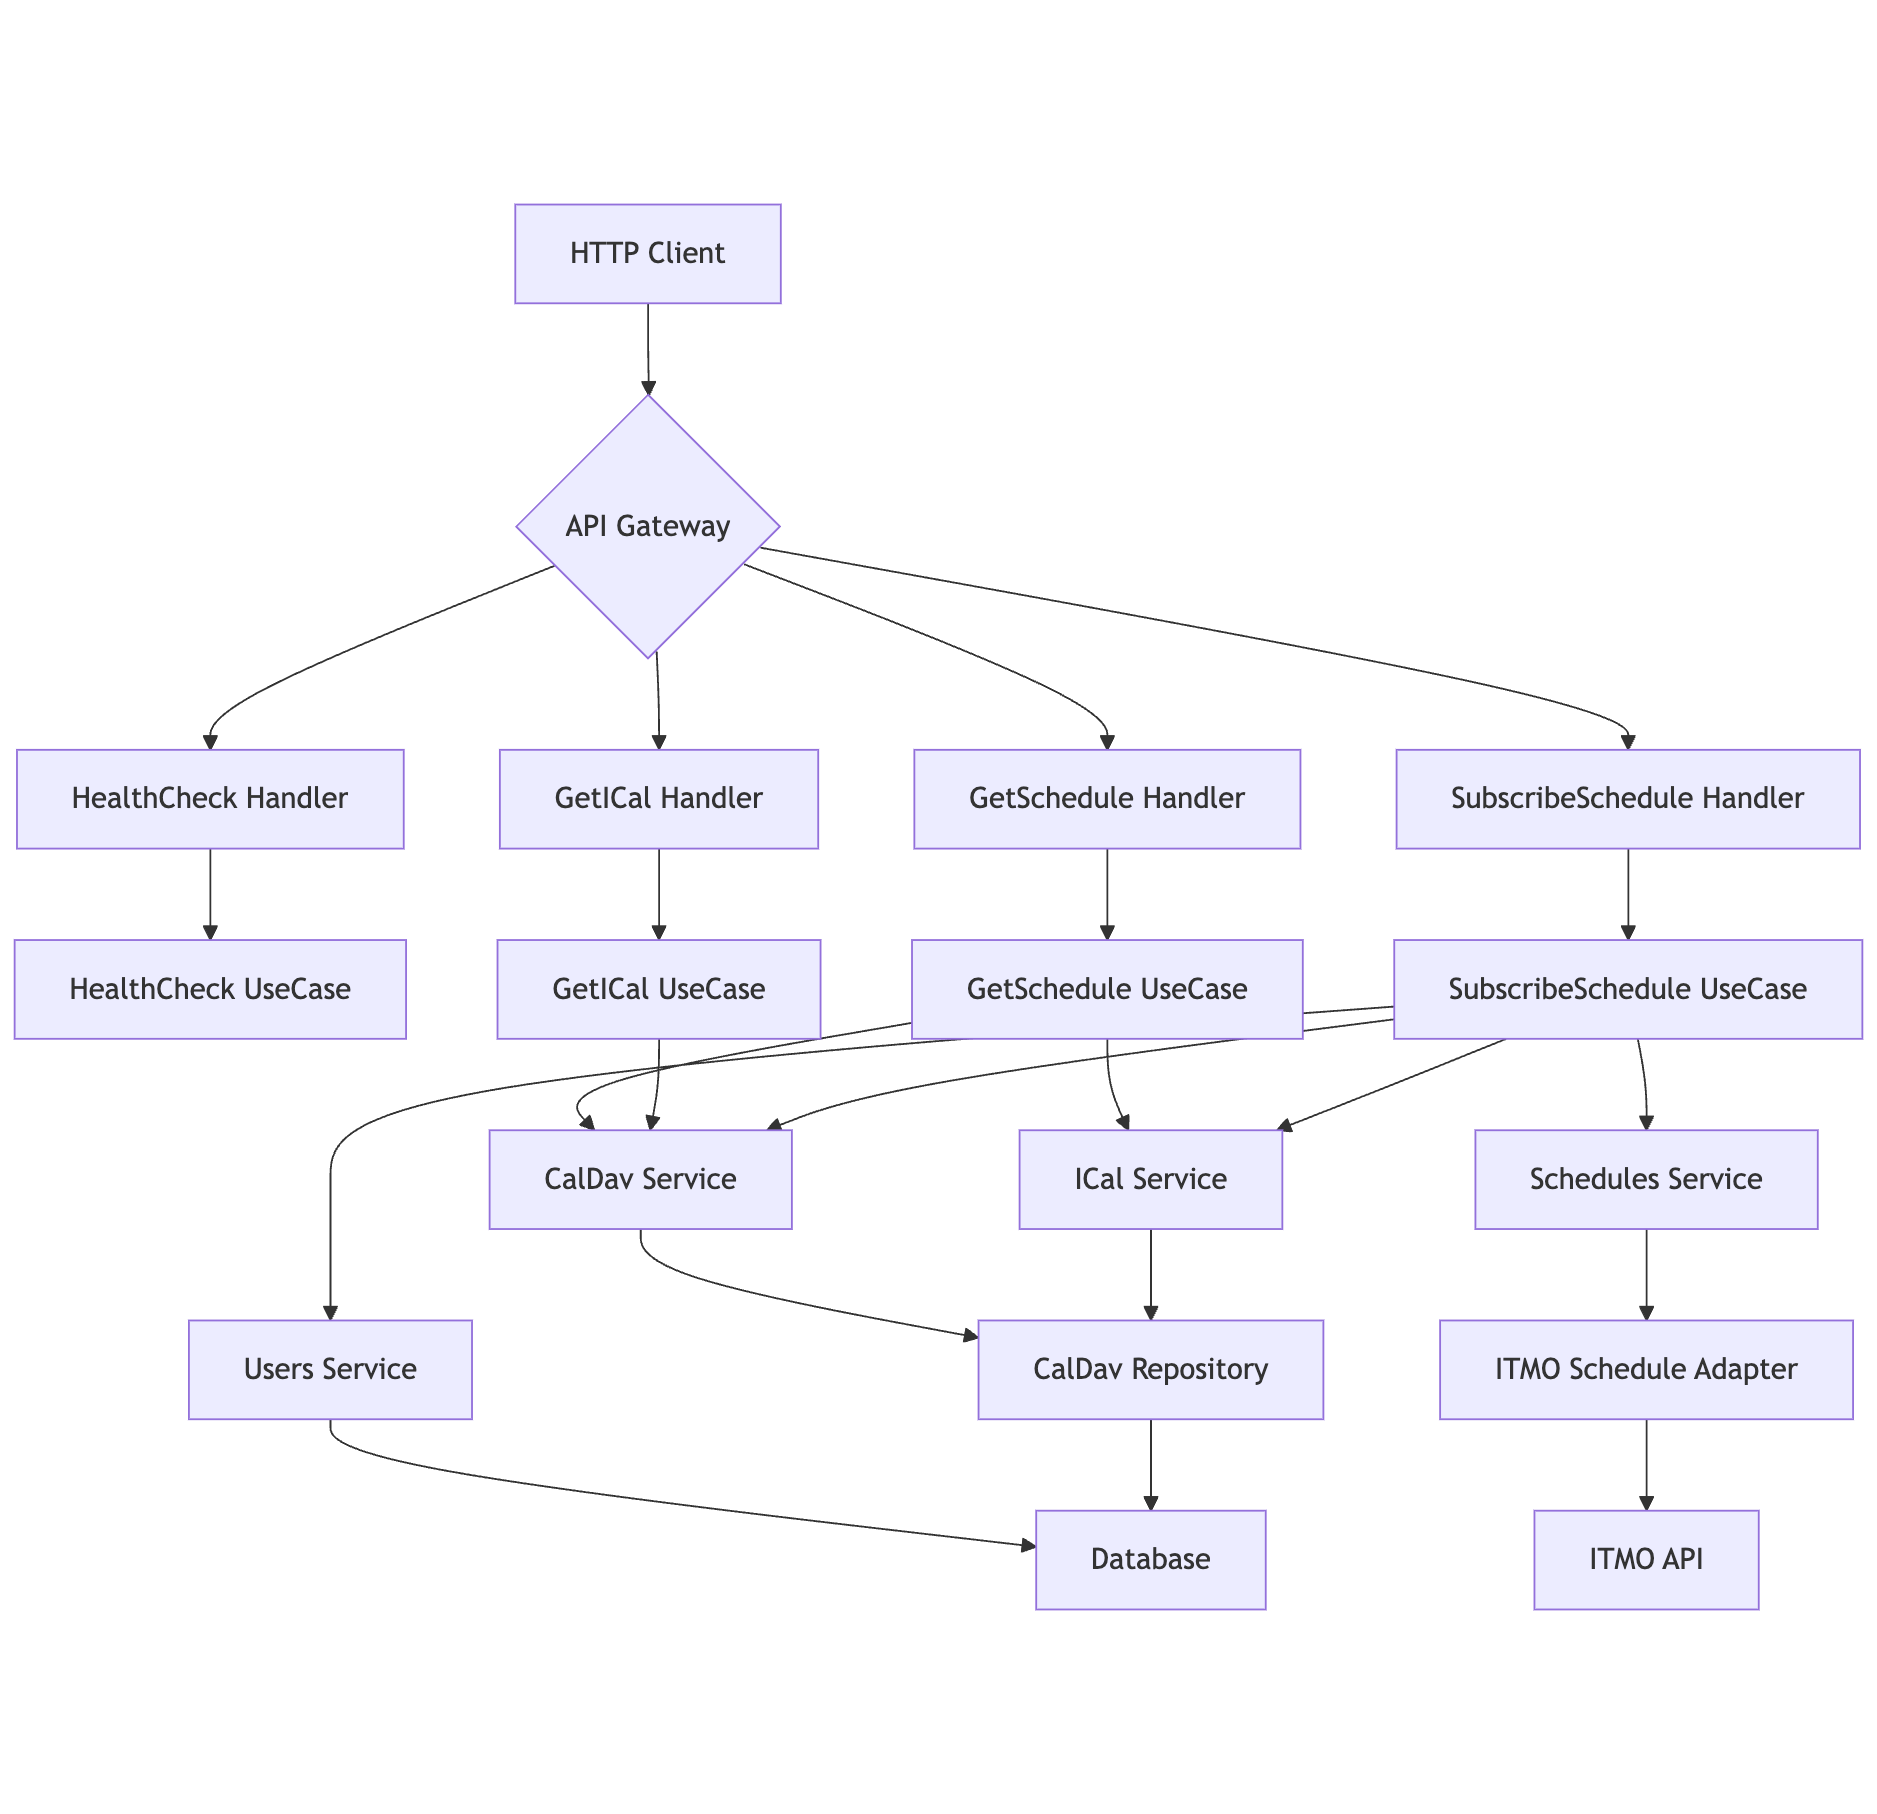
\includegraphics[width=0.6\textwidth]{images/mermaid-1.png}
\end{figure}

\paragraph{Пример Use Case: SubscribeSchedule}
Данный use case отвечает за регистрацию пользователя и создание/обновление его iCalendar файла.
\begin{figure}[h!]
    \centering
    \caption{Диаграмма последовательности для Use Case: SubscribeSchedule}
    \label{fig:subscribe-sequence}
    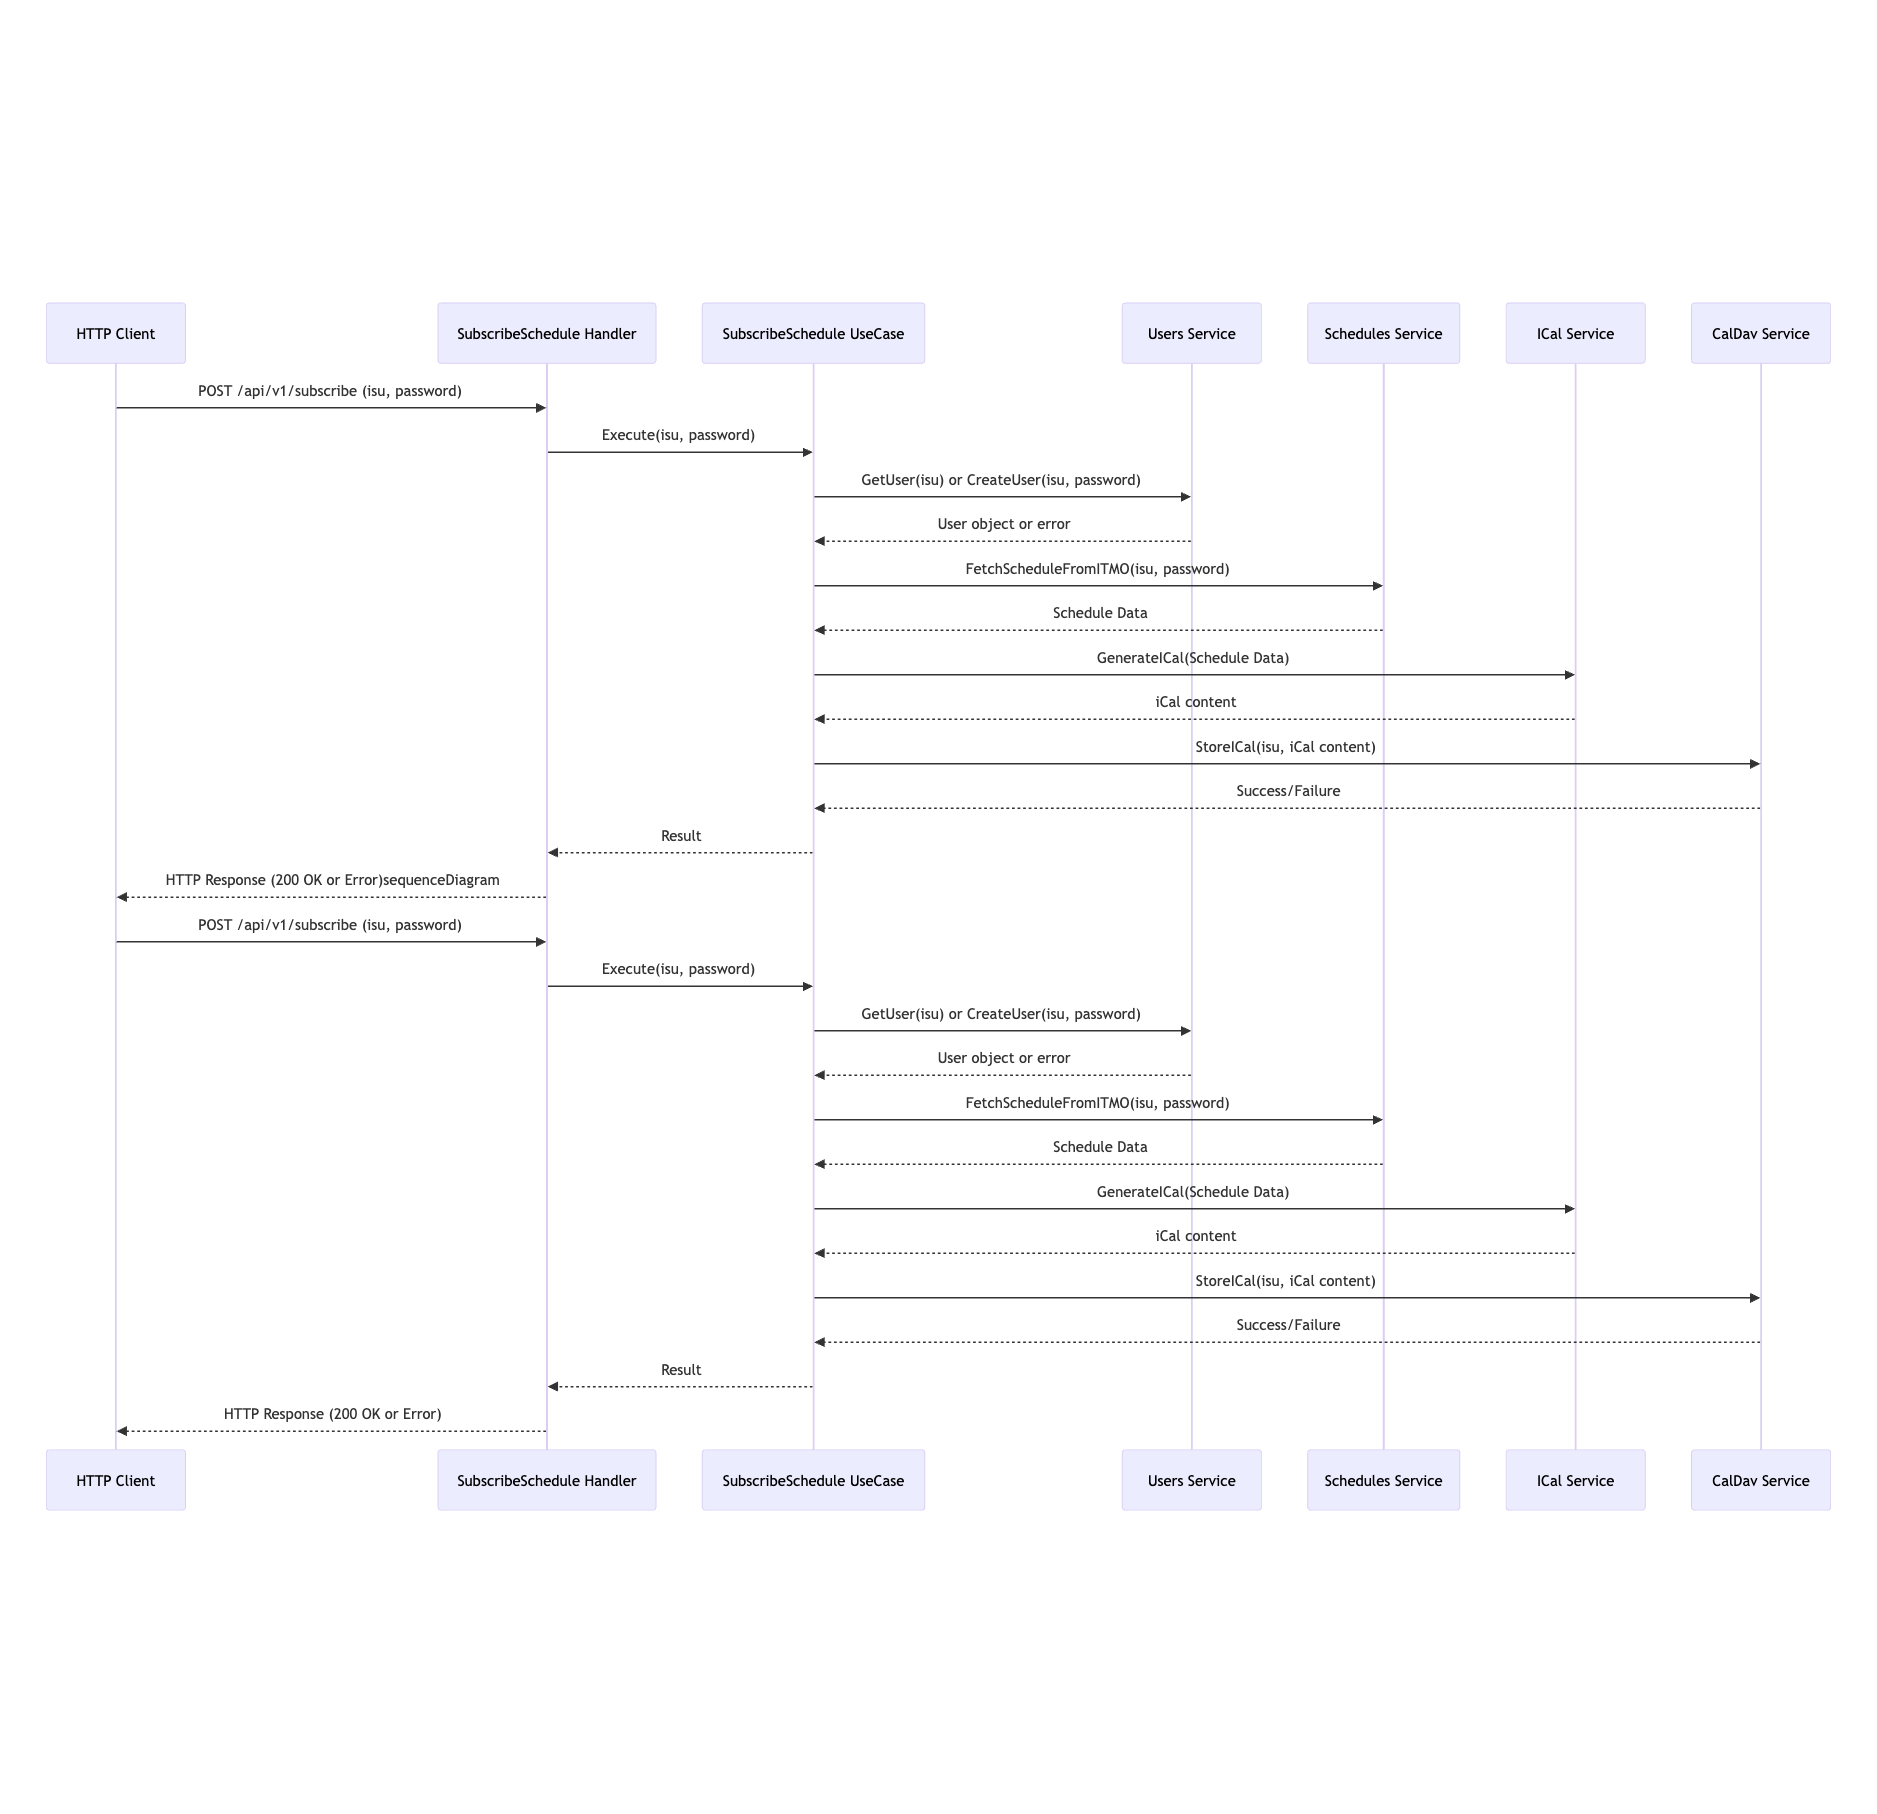
\includegraphics[width=0.6\textwidth]{images/mermaid-2.png}
\end{figure}

\subsection{Аспекты безопасности}
\begin{itemize}
    \item \textbf{Аутентификация}: Планируется использование JWT, что является стандартным подходом для защиты API.
    \item \textbf{Передача данных}: Swagger спецификация указывает на использование HTTPS (подразумевается, т.к. `basePath` не содержит схему, но `consumes` и `produces` `application/json` обычно передаются по HTTPS в production). Локально для разработки используется скрипт \texttt{generate-certs.sh} для создания самоподписанных сертификатов.
    \item \textbf{Обработка ошибок}: Сервис возвращает стандартизированные JSON-ответы об ошибках.
\end{itemize}

\section{Обзор архитектуры Flutter-приложения calendar-sync}
Мобильное приложение \texttt{calendar-sync} разработано на Flutter и предназначено для отображения расписания ИТМО и его синхронизации.

\subsection{Основные компоненты и структура}
Приложение использует следующие ключевые компоненты и подходы:
\begin{itemize}
    \item \textbf{State Management}: Пакет \texttt{provider} для управления состоянием и внедрения зависимостей (\texttt{ApiService}, \texttt{CalendarService}, \texttt{CalendarProvider}).
    \item \textbf{Навигация}: Используется именованная навигация с экранами \texttt{SplashScreen}, \texttt{WelcomeScreen}, \texttt{SyncScreen}.
    \item \textbf{Сервисы}:
    \begin{itemize}
        \item \texttt{ApiService}: Отвечает за все взаимодействия с backend API (запросы на подписку, получение расписания). Включает обработку самоподписанных сертификатов для локальной разработки.
        \item \texttt{CalendarService}: Предположительно, отвечает за взаимодействие с нативными календарями устройства (хотя детали его реализации не были проанализированы в данном отчете).
    \end{itemize}
    \item \textbf{Модели}: \texttt{CalendarEvent} для представления событий расписания.
    \item \textbf{UI}: Стандартные виджеты Flutter, кастомная тема оформления.
\end{itemize}

\begin{figure}[h!]
    \centering
    \caption{Упрощенная схема работы Flutter-приложения calendar-sync}
    \label{fig:flutter-flow}
    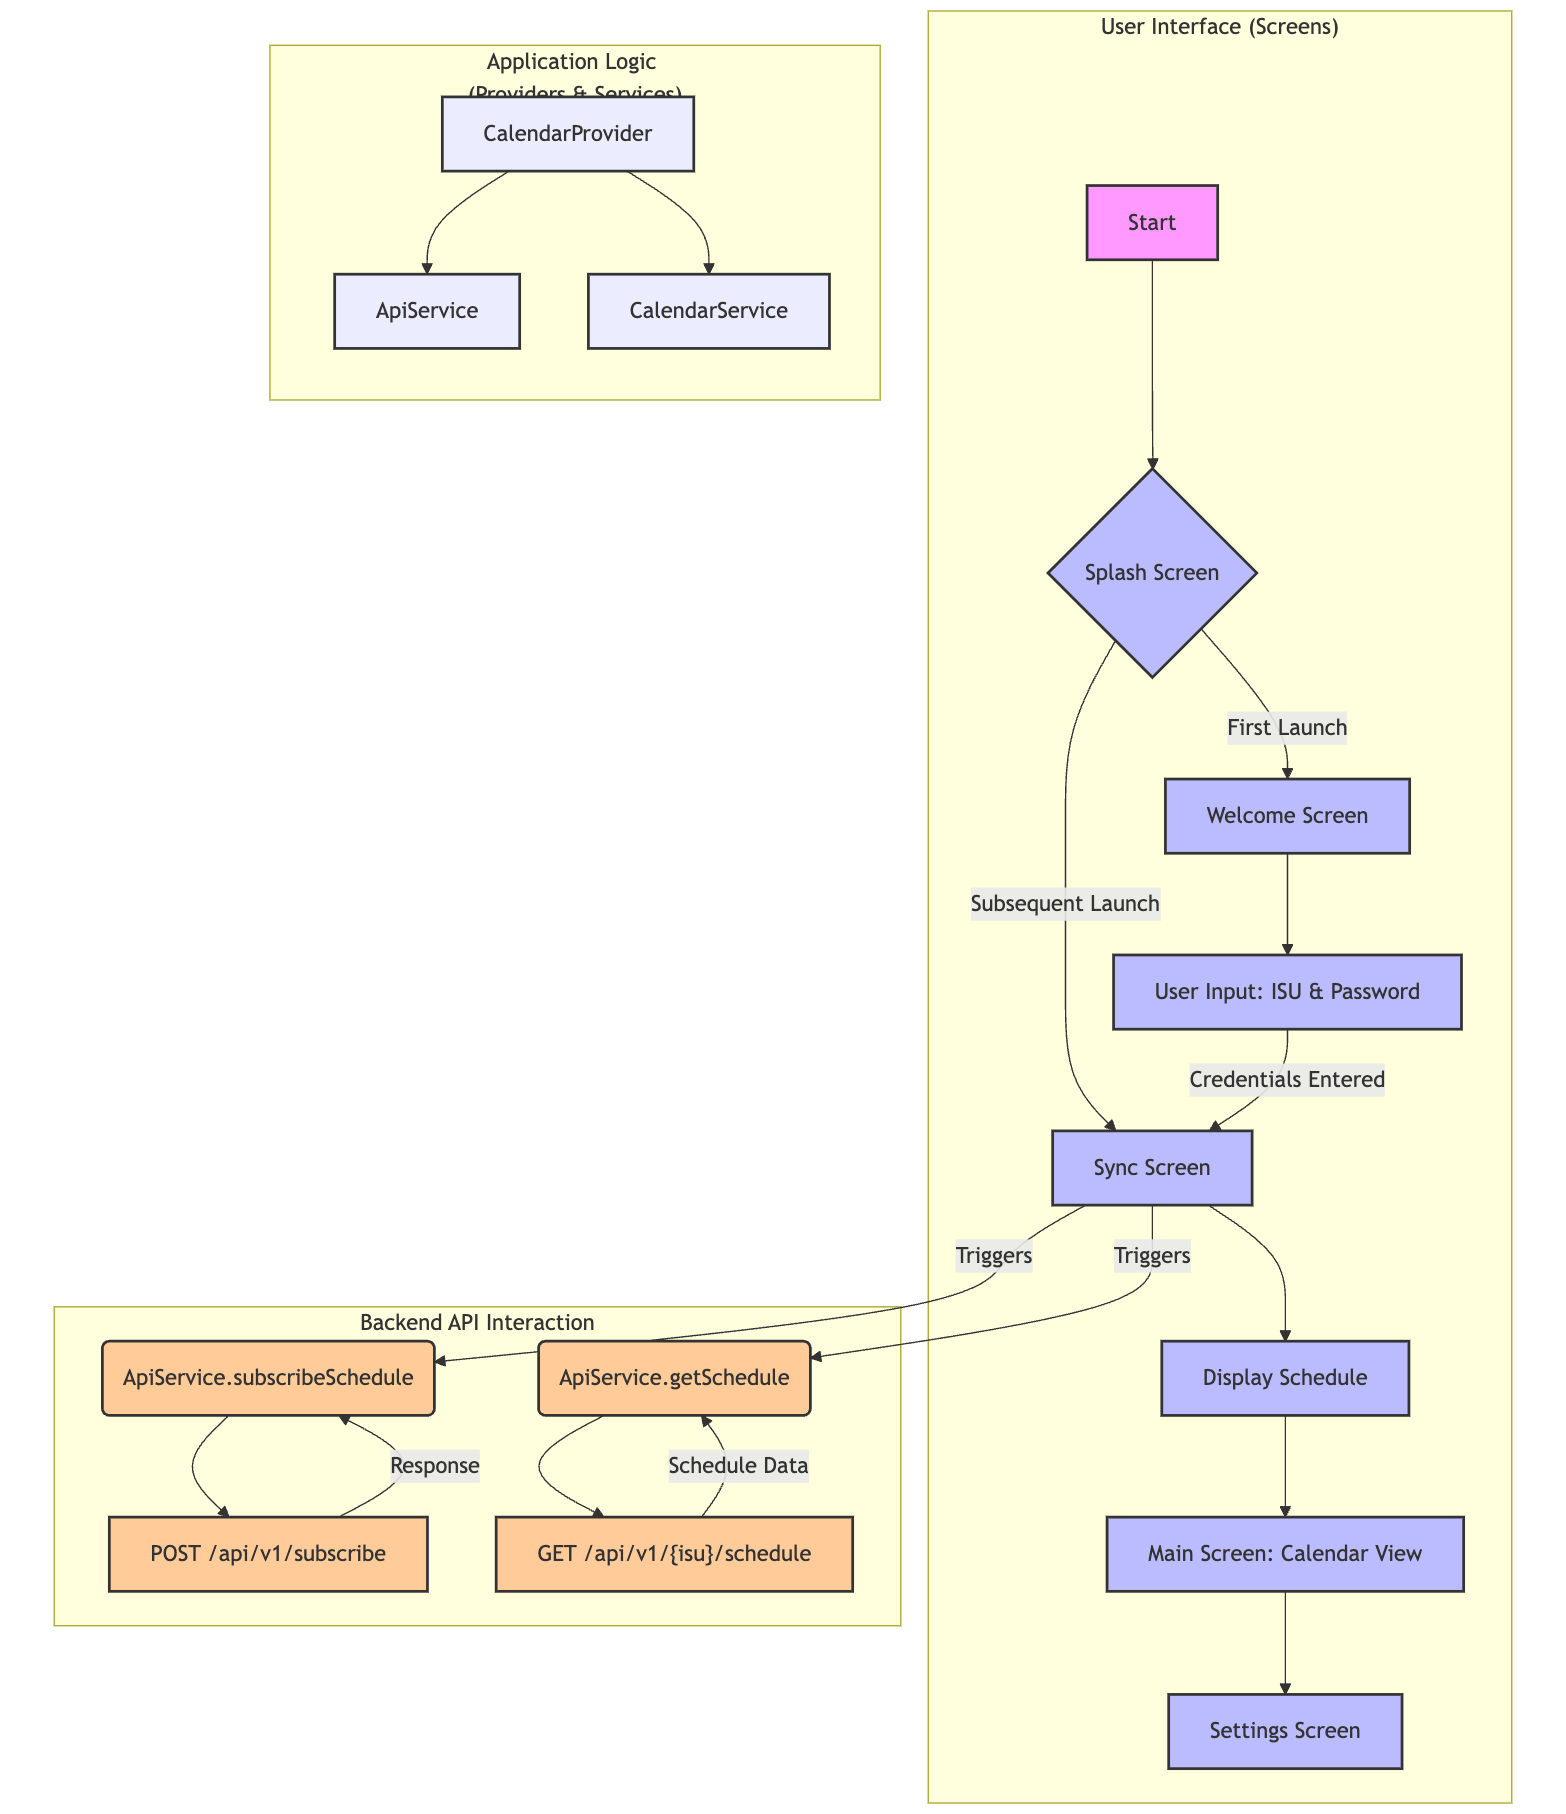
\includegraphics[width=0.6\textwidth]{images/mermaid-3.png}
\end{figure}

\subsection{Реализация запрета на создание скриншотов}
В файле \texttt{lib/main.dart} используется пакет \texttt{screen\_protector} для запрета создания скриншотов. Функция \texttt{\_enableScreenshotBlocking} вызывает \texttt{ScreenProtector.protectDataLeakageWithBlur()} для Android и iOS. Это соответствует требованию лабораторной работы.

\begin{minted}{dart}
Future<void> _enableScreenshotBlocking() async {
  if (defaultTargetPlatform == TargetPlatform.android || 
      defaultTargetPlatform == TargetPlatform.iOS) {
    try {
      await ScreenProtector.protectDataLeakageWithBlur();
    } catch (e) {
      if (kDebugMode) {
        print('Screenshot blocking not supported: $e');
      }
    }
  } else {
    if (kDebugMode) {
      print('Screenshot blocking skipped for desktop');
    }
  }
}
\end{minted}

\subsection{Взаимодействие с backend}
Класс \texttt{ApiService} (\texttt{lib/services/api\_service.dart}) инкапсулирует логику HTTP-запросов к backend. Примечательной особенностью является обработка самоподписанных SSL-сертификатов, что важно для тестирования с локально развернутым backend.
\begin{minted}{dart}
// Фрагмент из ApiService для обработки сертификатов
http.Client _createHttpClient() {
  final httpClient = HttpClient();
  httpClient.badCertificateCallback = 
    (X509Certificate cert, String host, int port) {
    print('Warning: Accepting certificate for $host:$port');
    return true; // Принимаем самоподписанный сертификат
  };
  httpClient.connectionTimeout = const Duration(seconds: 30);
  return IOClient(httpClient);
}
\end{minted}
Это упрощает разработку, но в production-сборке такой подход должен быть заменен на проверку валидных сертификатов.

\section{Анализ APK файлов}
В рамках лабораторной работы были выполнены сборка, декомпиляция и анализ APK-файлов приложения.

\subsection{Получение APK с обфускацией и без}
Были собраны два APK-файла:
\begin{itemize}
    \item \texttt{app-release.apk}: с включенной обфускацией кода (стандартный release-режим Flutter).
    \item \texttt{app-release-no-obfuscate.apk}: предположительно, собран с флагами для минимизации или отключения обфускации (например, \texttt{--no-shrink}).
\end{itemize}
Команды для сборки:
\begin{minted}{bash}
# Сборка с обфускацией (стандартный релиз)
flutter build apk --release

# Сборка без обфускации (или с минимальной)
flutter build apk --release --no-shrink 
# (Примечание: --no-shrink влияет на R8/ProGuard, 
# Dart код обфусцируется самим Flutter)
\end{minted}


\subsection{Декомпиляция APK}
Оба APK-файла были декомпилированы с помощью ApkTool.
\begin{minted}{bash}
apktool d app-release.apk -o report/apks/decompiled-release
apktool d app-release-no-obfuscate.apk -o report/apks/decompiled-no-obfuscate
\end{minted}
Сравнение результатов декомпиляции (файл \texttt{report/apks/diff.txt}) показывает различия, связанные с обфускацией имен классов, методов и полей в smali-коде, а также возможные различия в ресурсах из-за оптимизаций R8.

\textbf{Выдержка из diff-файла (\texttt{report/apks/diff.txt}):}
\begin{small} % Уменьшаем шрифт для содержимого файла
\lstinputlisting[basicstyle=\ttfamily\tiny, breaklines=true, showstringspaces=false]{apks/diff.txt}
\end{small}


\subsection{Сканирование утилитой apkleaks}
Приложение было просканировано утилитой \texttt{apkleaks} для поиска потенциальных утечек чувствительной информации.
\begin{minted}{bash}
apkleaks -f report/apks/app-release.apk -o report/apks/appleaks-result.txt
\end{minted}
Результаты сканирования сохранены в файле \texttt{report/apks/appleaks-result.txt}.

\textbf{Содержимое файла \texttt{report/apks/appleaks-result.txt}:}
\begin{small} % Уменьшаем шрифт для содержимого файла
\lstinputlisting[basicstyle=\ttfamily\tiny, breaklines=true, showstringspaces=false]{apks/appleaks-result.txt}
\end{small}
Как правило, \texttt{apkleaks} может обнаружить URL-адреса, ключи API (если они захардкожены), email и другие строки, которые могут представлять интерес. В данном случае, он мог обнаружить \texttt{https://localhost/api/v1}.

\subsection{Проверка через VirusTotal}
APK-файл \texttt{app-release.apk} был проверен через сервис VirusTotal.
\begin{figure}[h!]
    \centering
    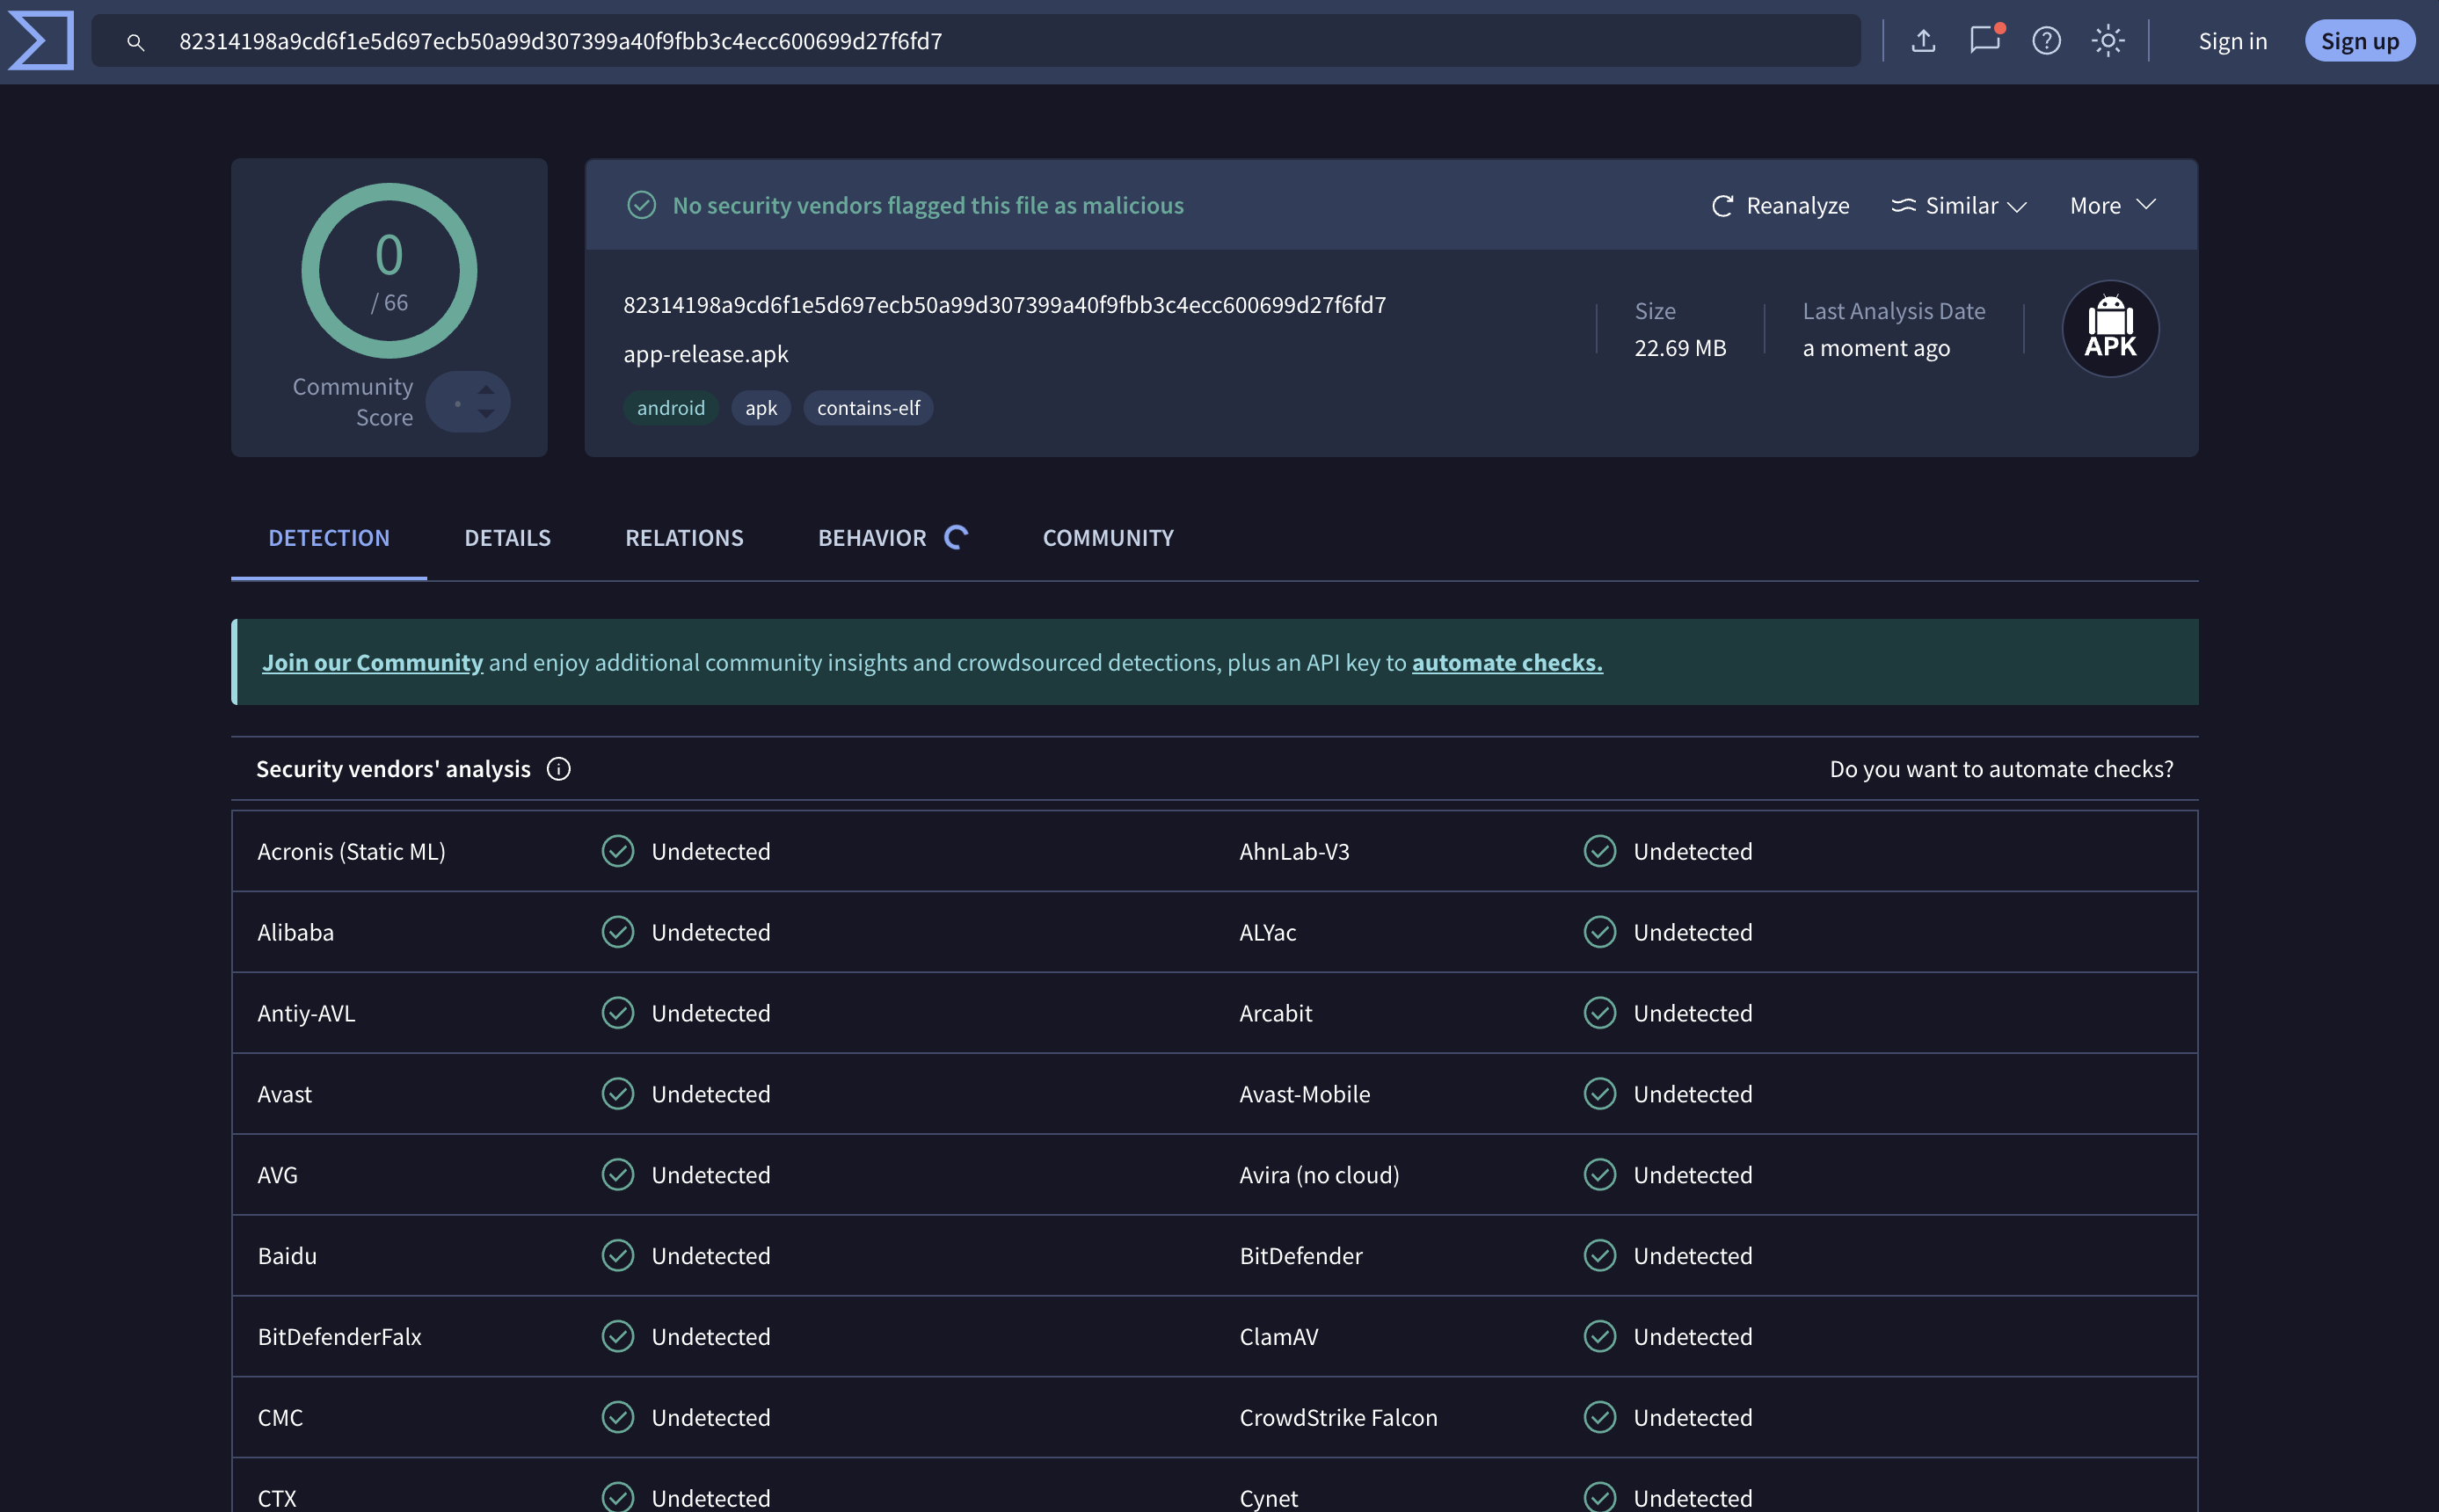
\includegraphics[width=0.9\textwidth]{images/virustotal.png}
    \caption{Результат проверки APK на VirusTotal}
    \label{fig:virustotal}
\end{figure}
Результаты показывают, что большинство антивирусных движков не обнаружили угроз (типично для большинства Flutter-приложений, если не используется специфический вредоносный код).

\section{Скриншоты работы Flutter-приложения}
Далее представлены скриншоты, демонстрирующие работу разработанного Flutter-приложения \texttt{calendar-sync}.

\begin{figure}[h!]
    \centering
    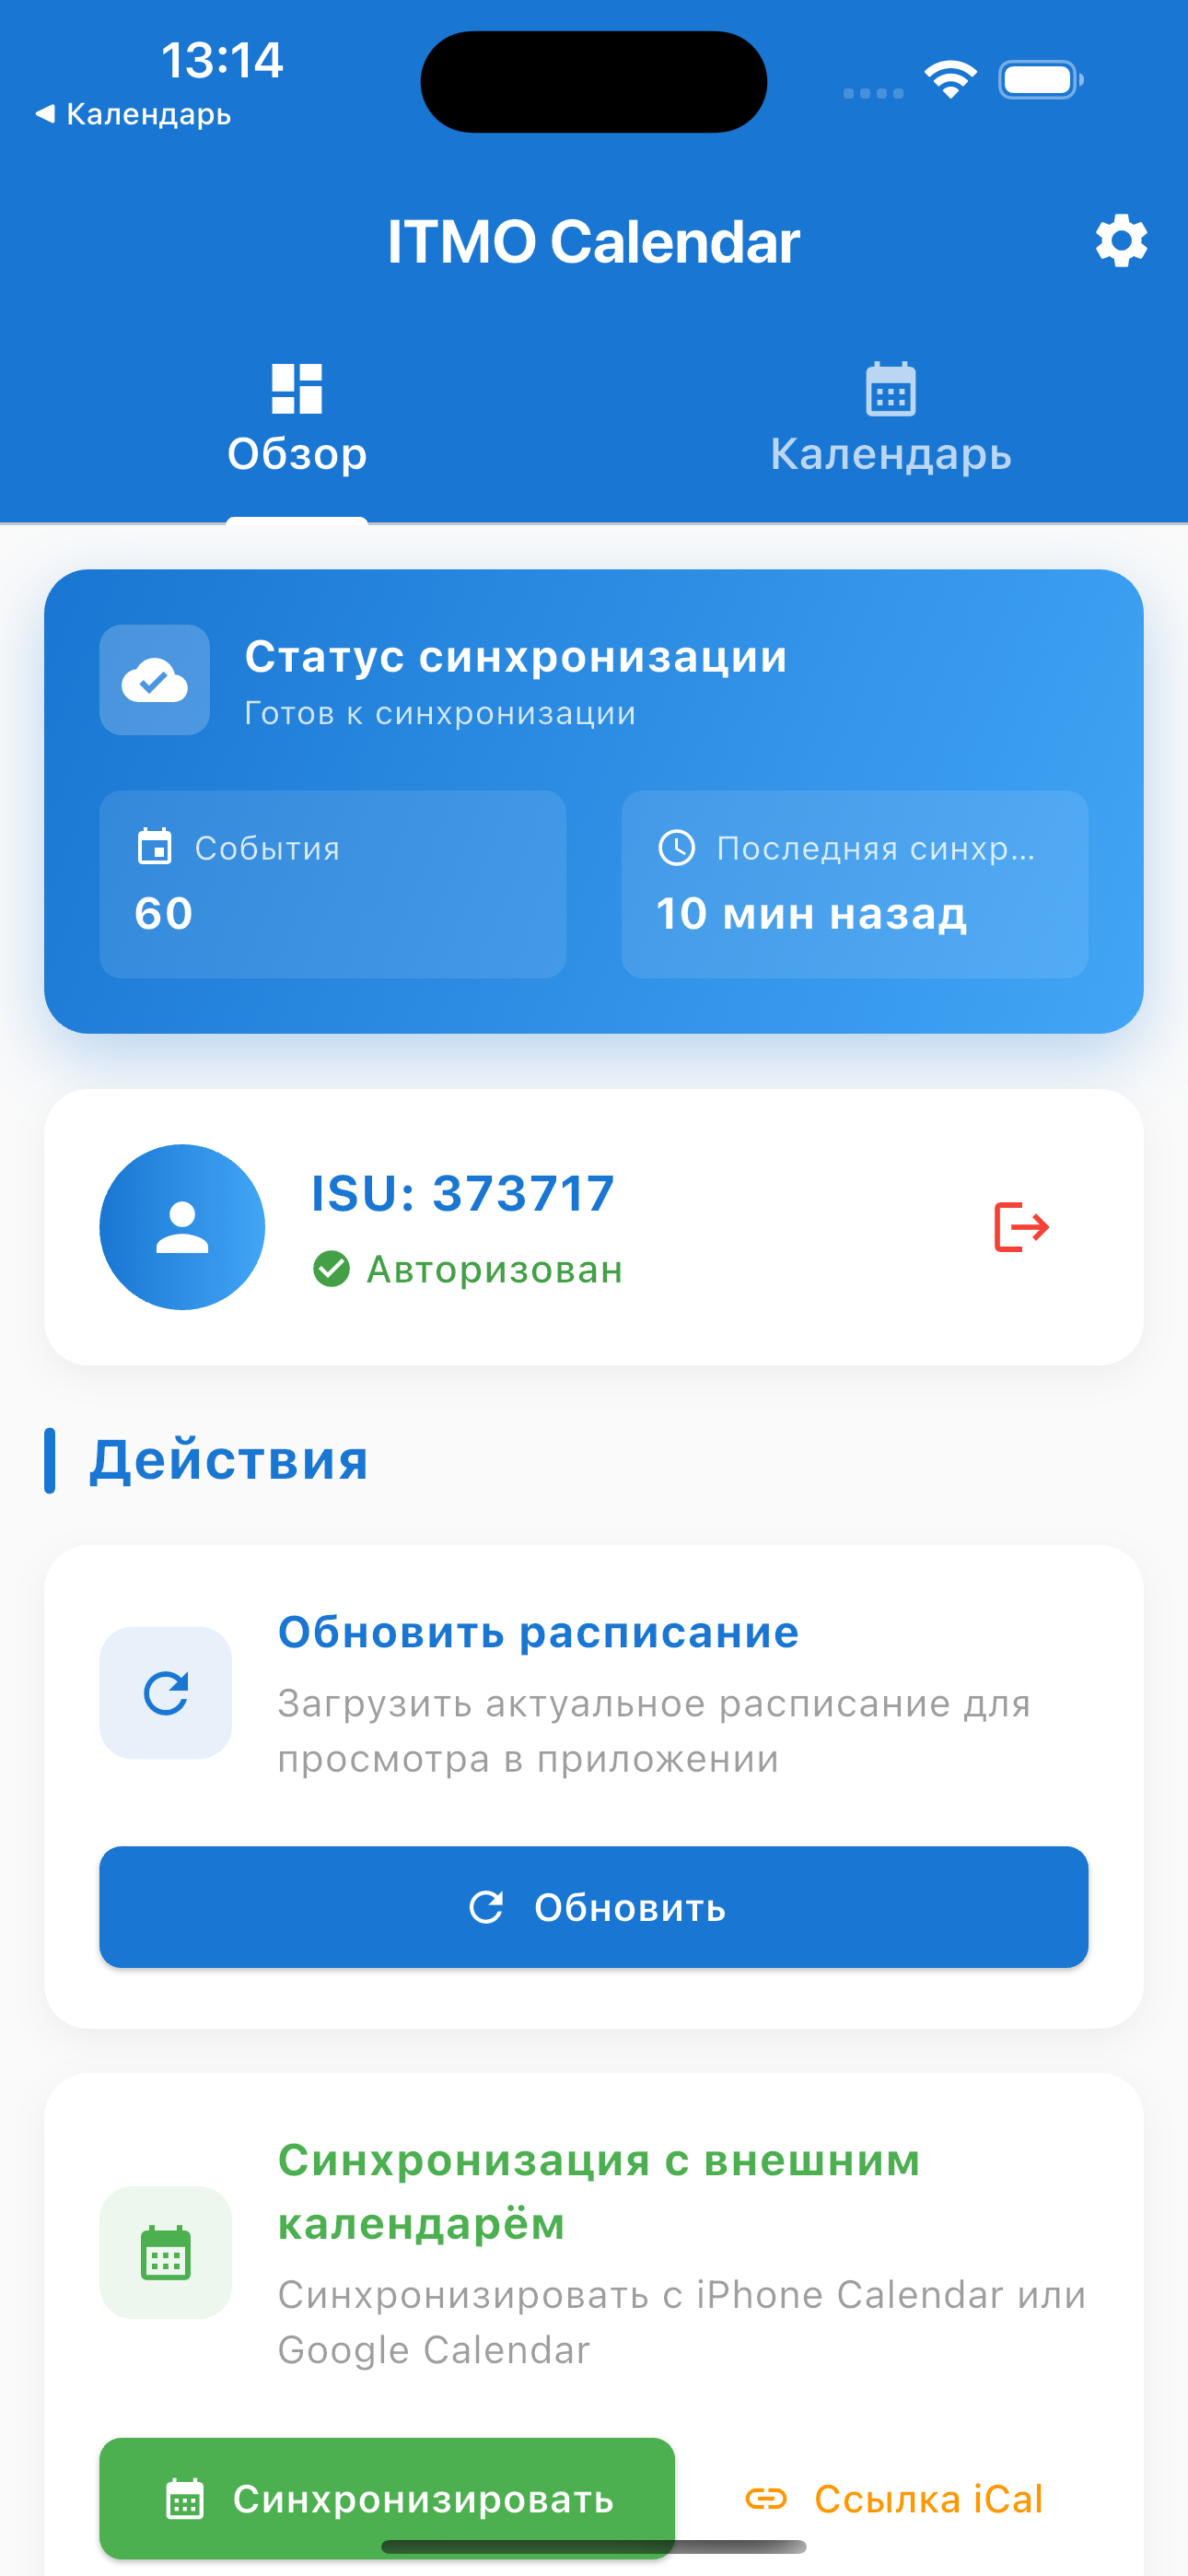
\includegraphics[width=0.6\textwidth]{images/main-screen.png}
    \caption{Главный экран приложения}
    \label{fig:main-screen}
\end{figure}

\begin{figure}[h!]
    \centering
    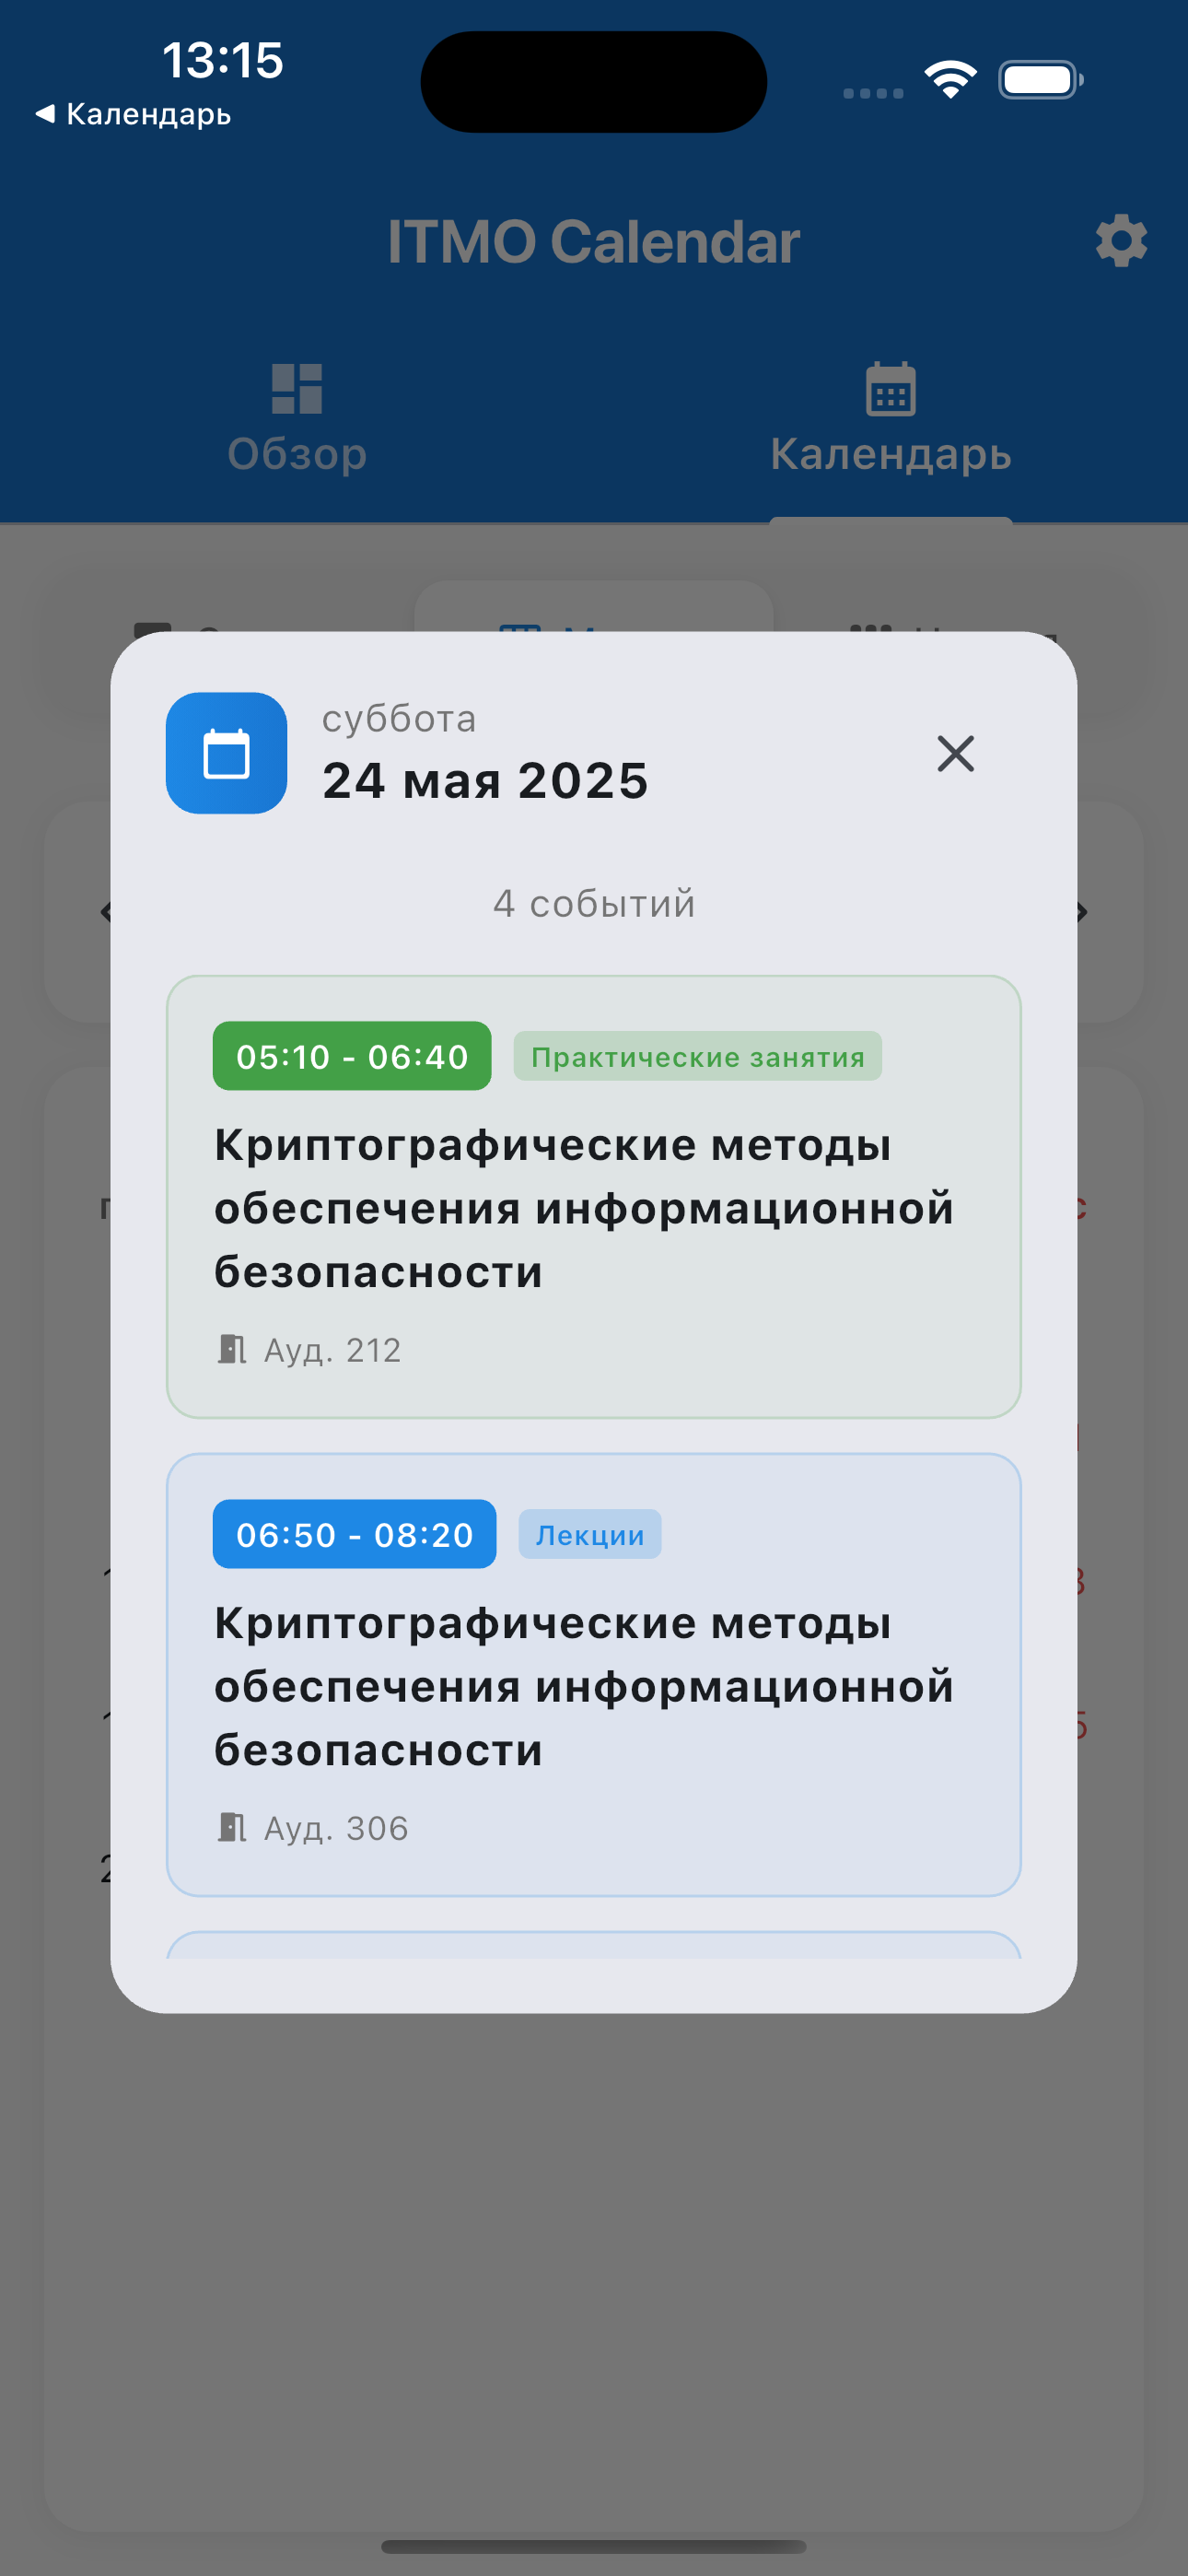
\includegraphics[width=0.6\textwidth]{images/calendar-month.png}
    \caption{Вид календаря на месяц}
    \label{fig:calendar-month}
\end{figure}

\begin{figure}[h!]
    \centering
    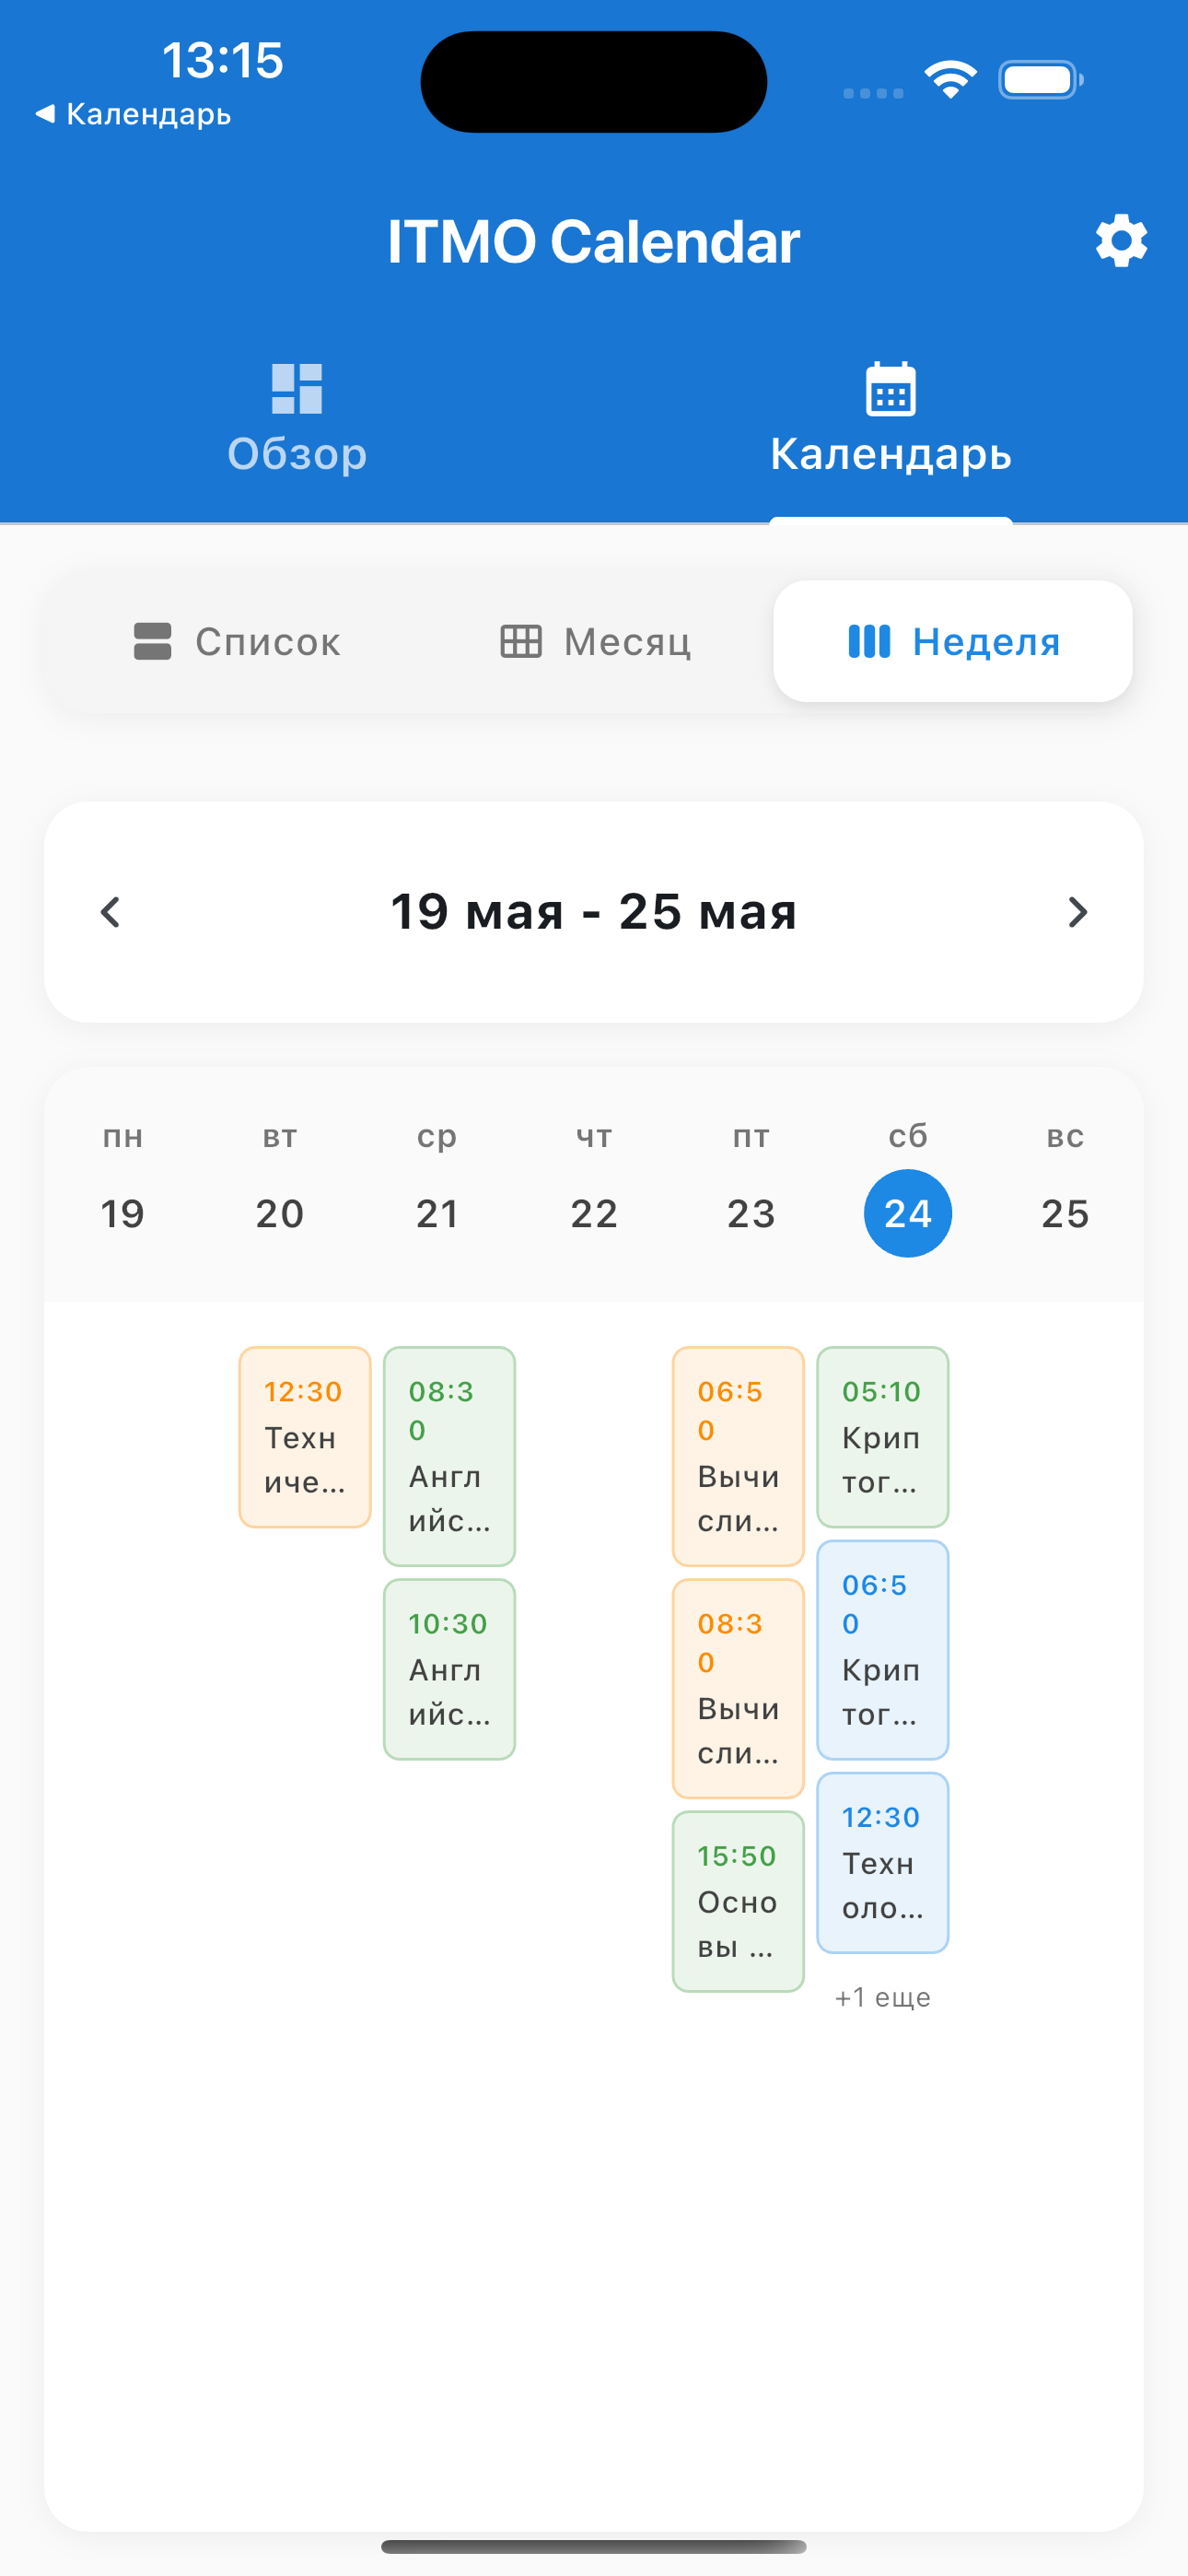
\includegraphics[width=0.6\textwidth]{images/calendar-week.png}
    \caption{Вид календаря на неделю}
    \label{fig:calendar-week}
\end{figure}

\begin{figure}[h!]
    \centering
    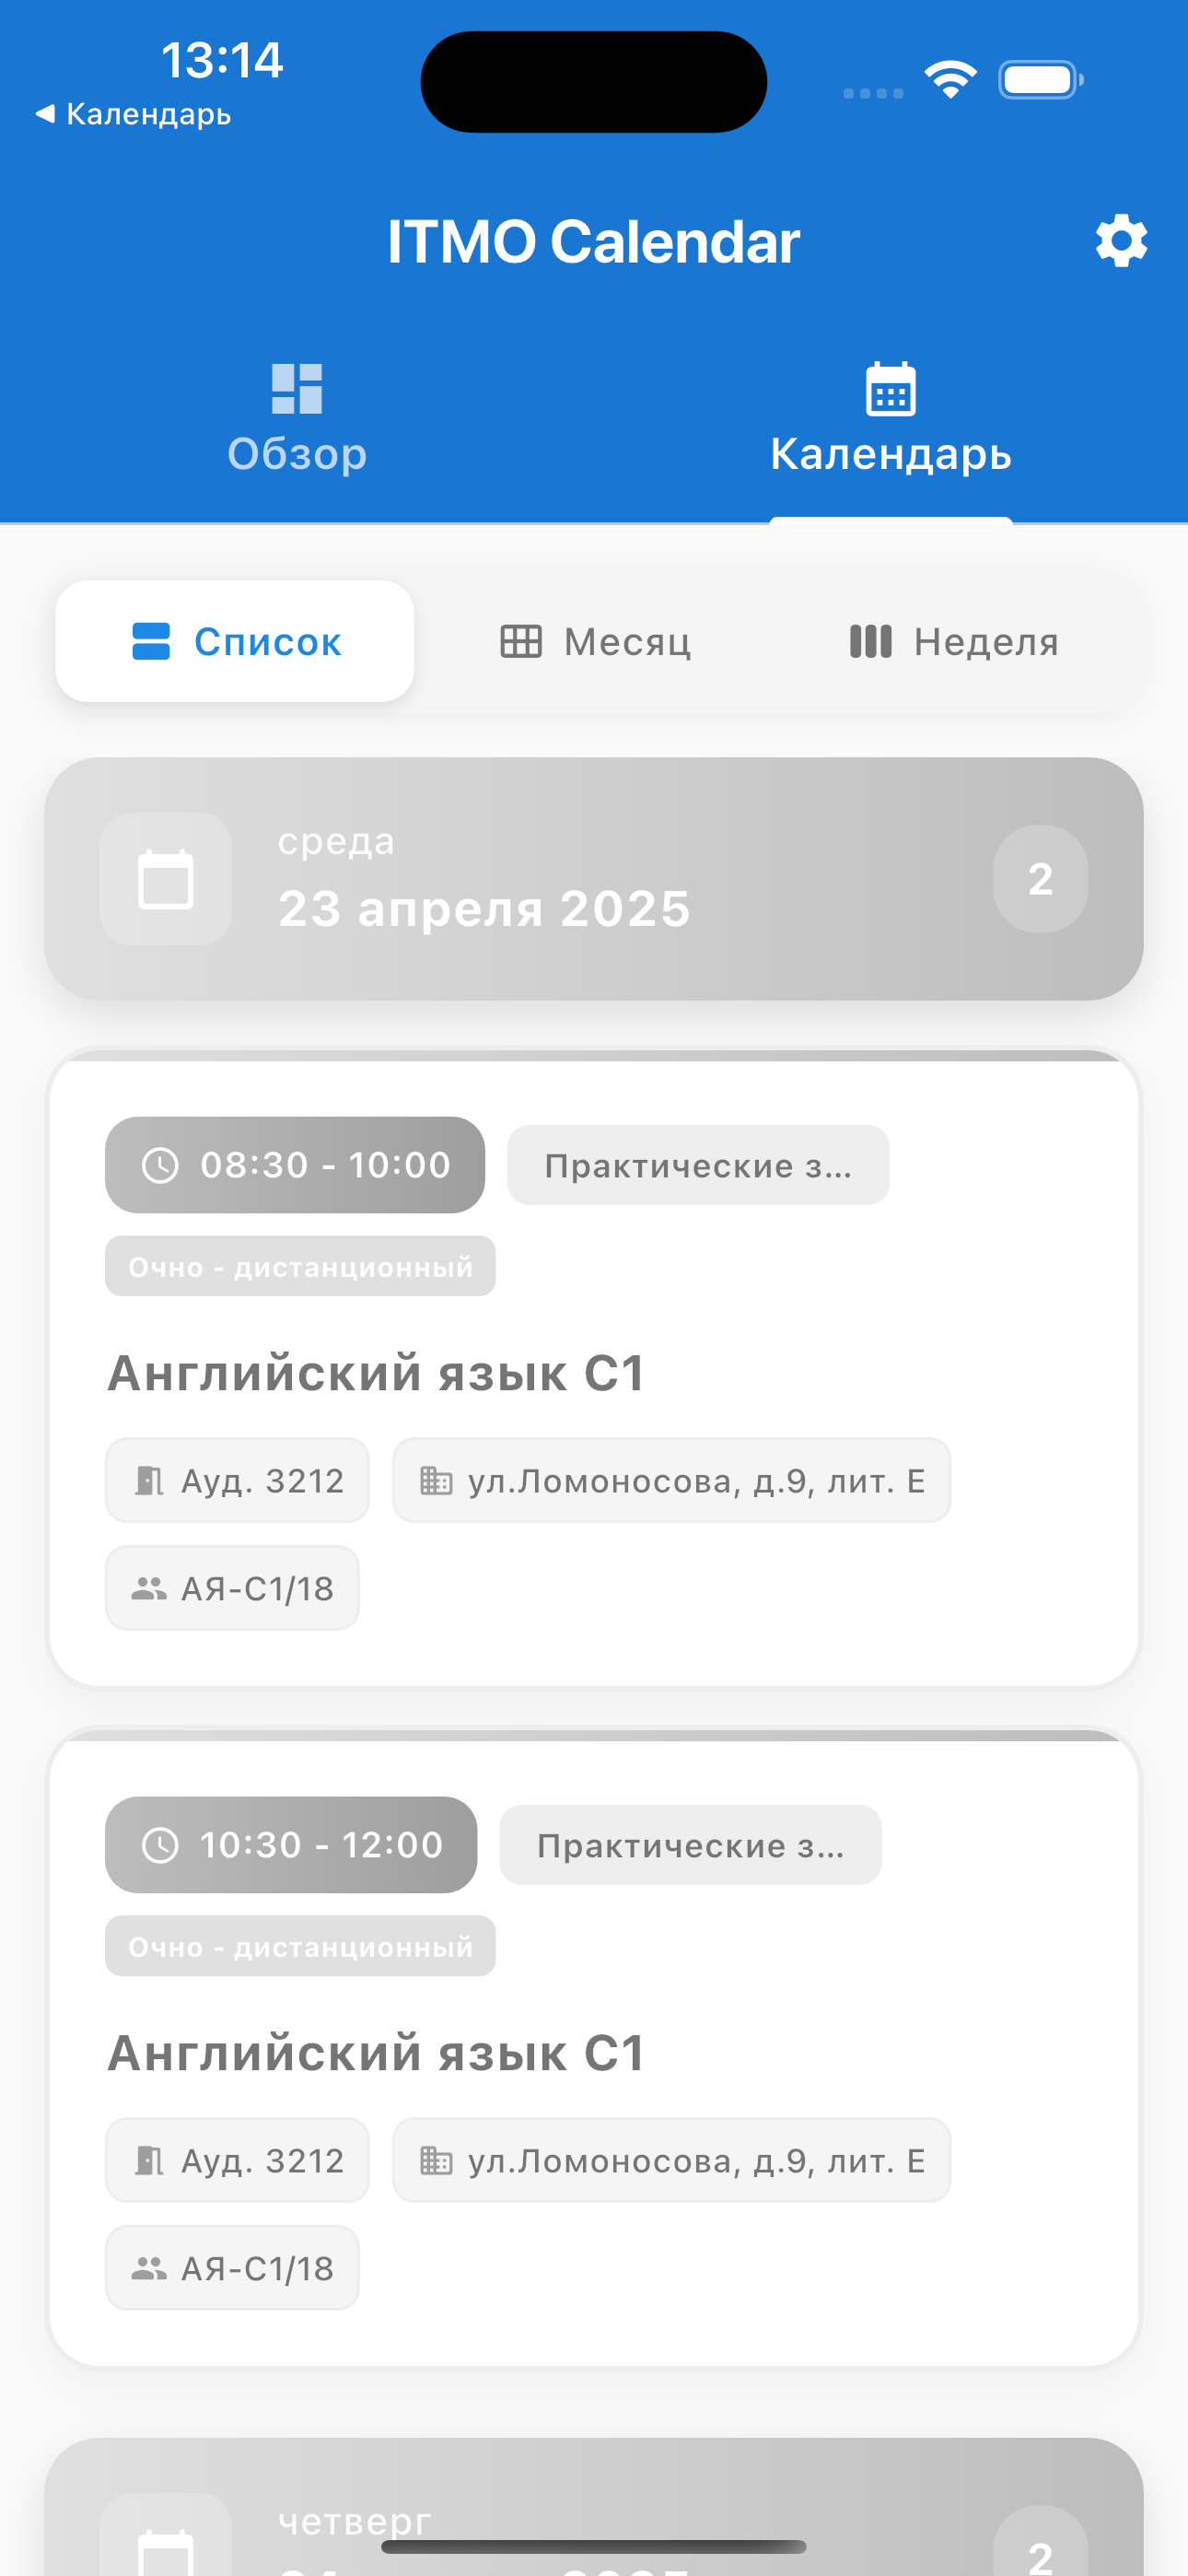
\includegraphics[width=0.6\textwidth]{images/calendar-list.png}
    \caption{Список событий}
    \label{fig:calendar-list}
\end{figure}

\begin{figure}[h!]
    \centering
    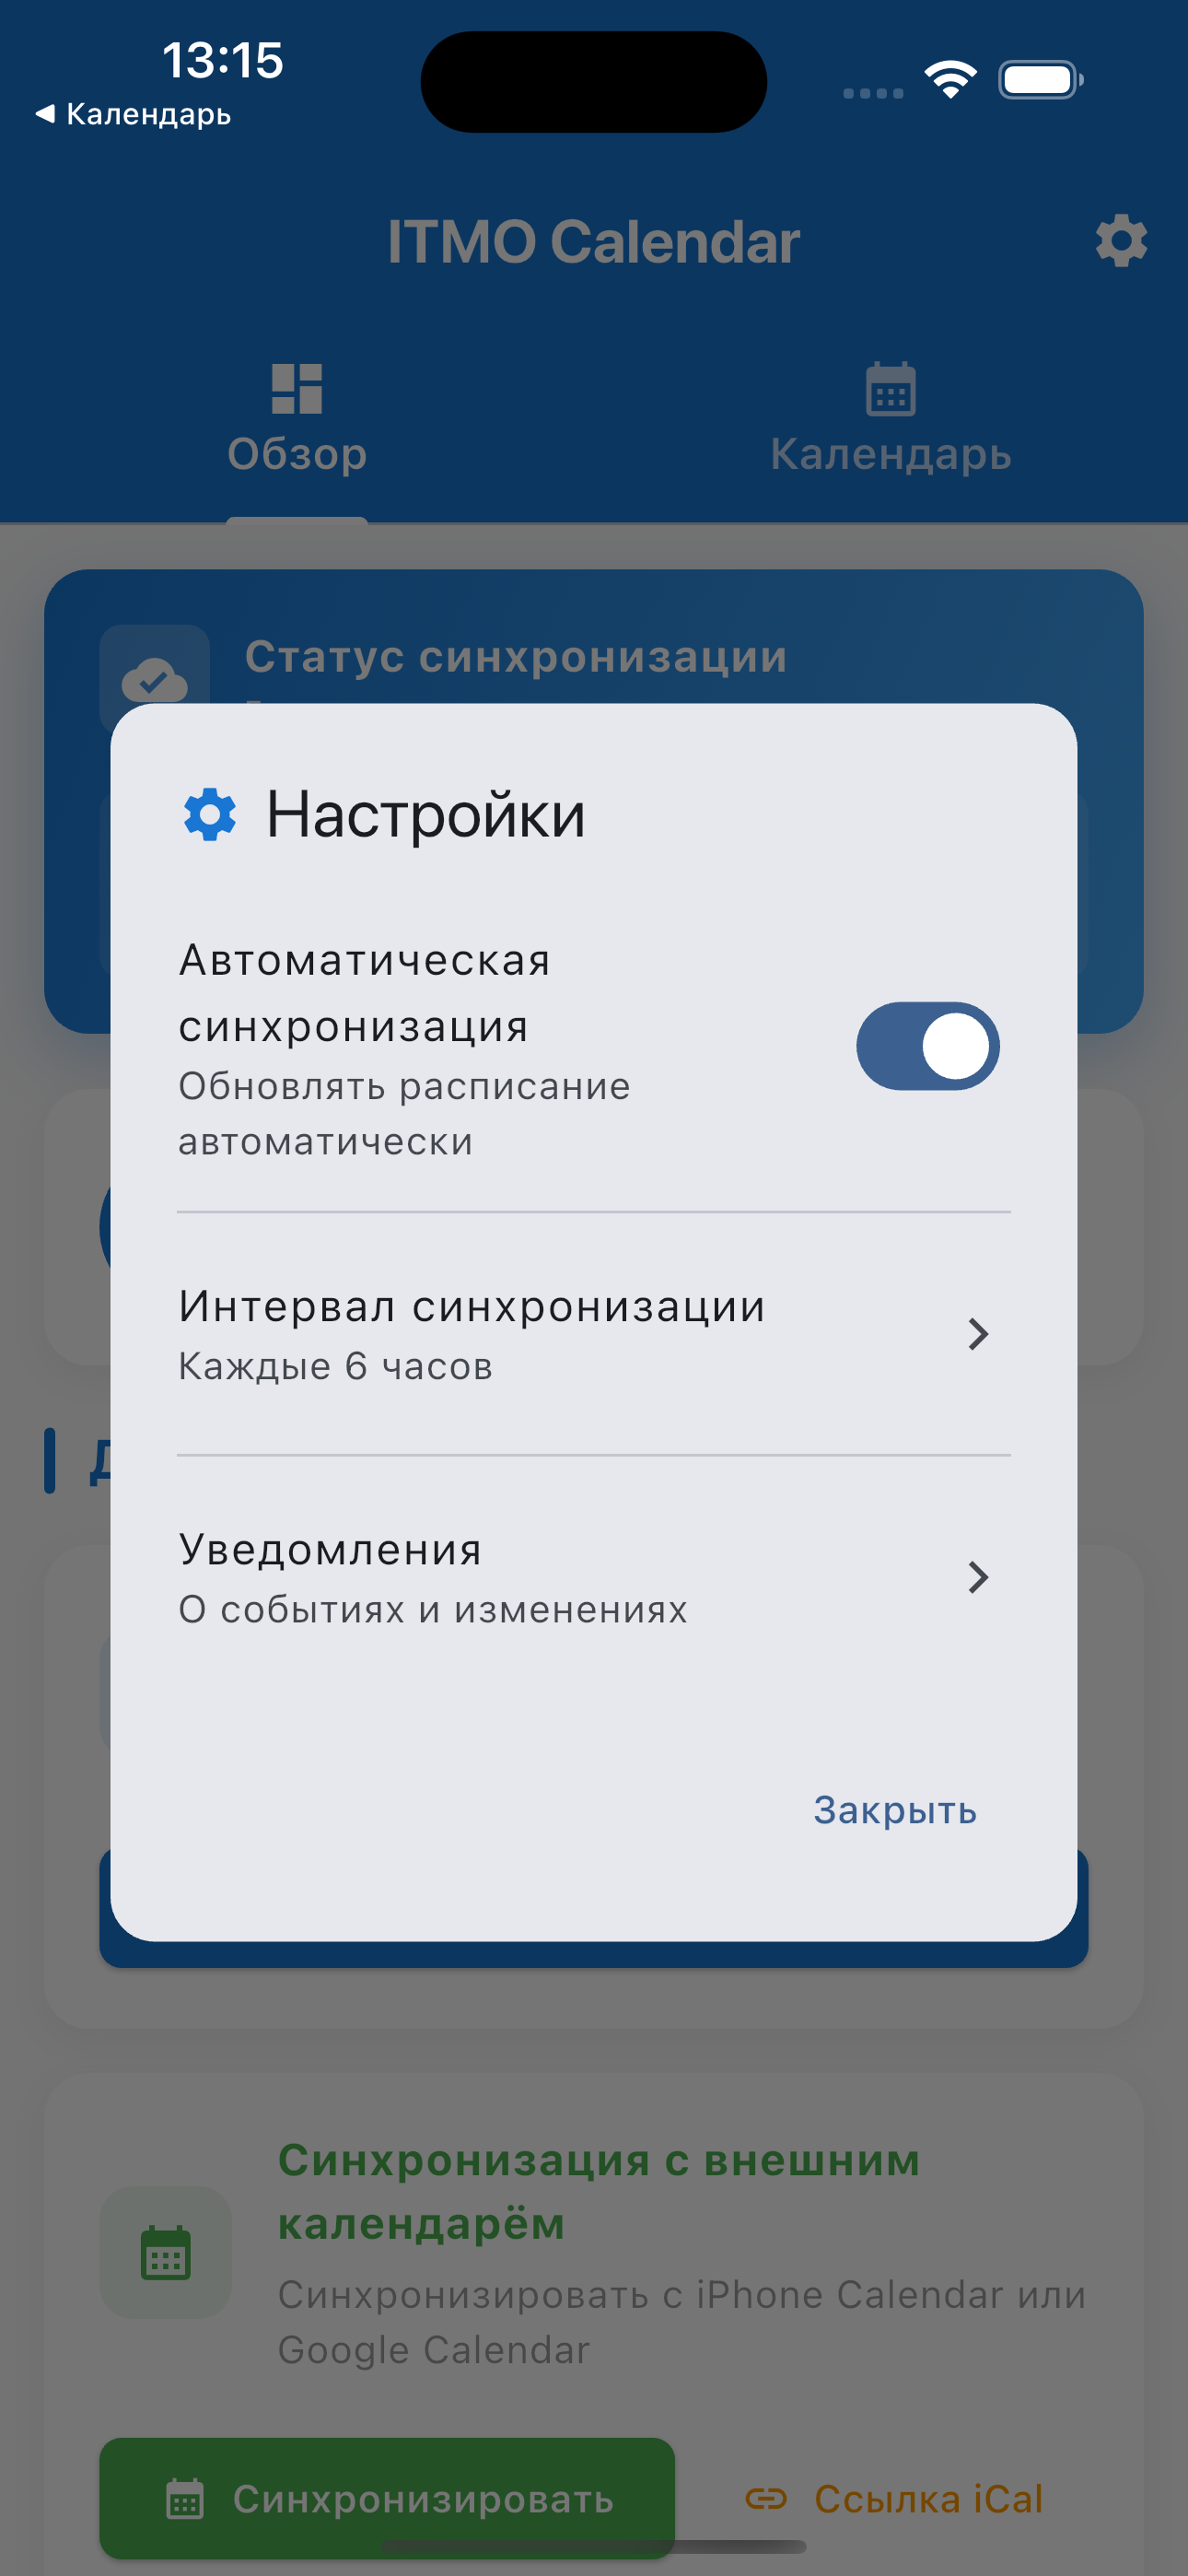
\includegraphics[width=0.6\textwidth]{images/settings.png}
    \caption{Экран настроек}
    \label{fig:settings}
\end{figure}

\begin{figure}[h!]
    \centering
    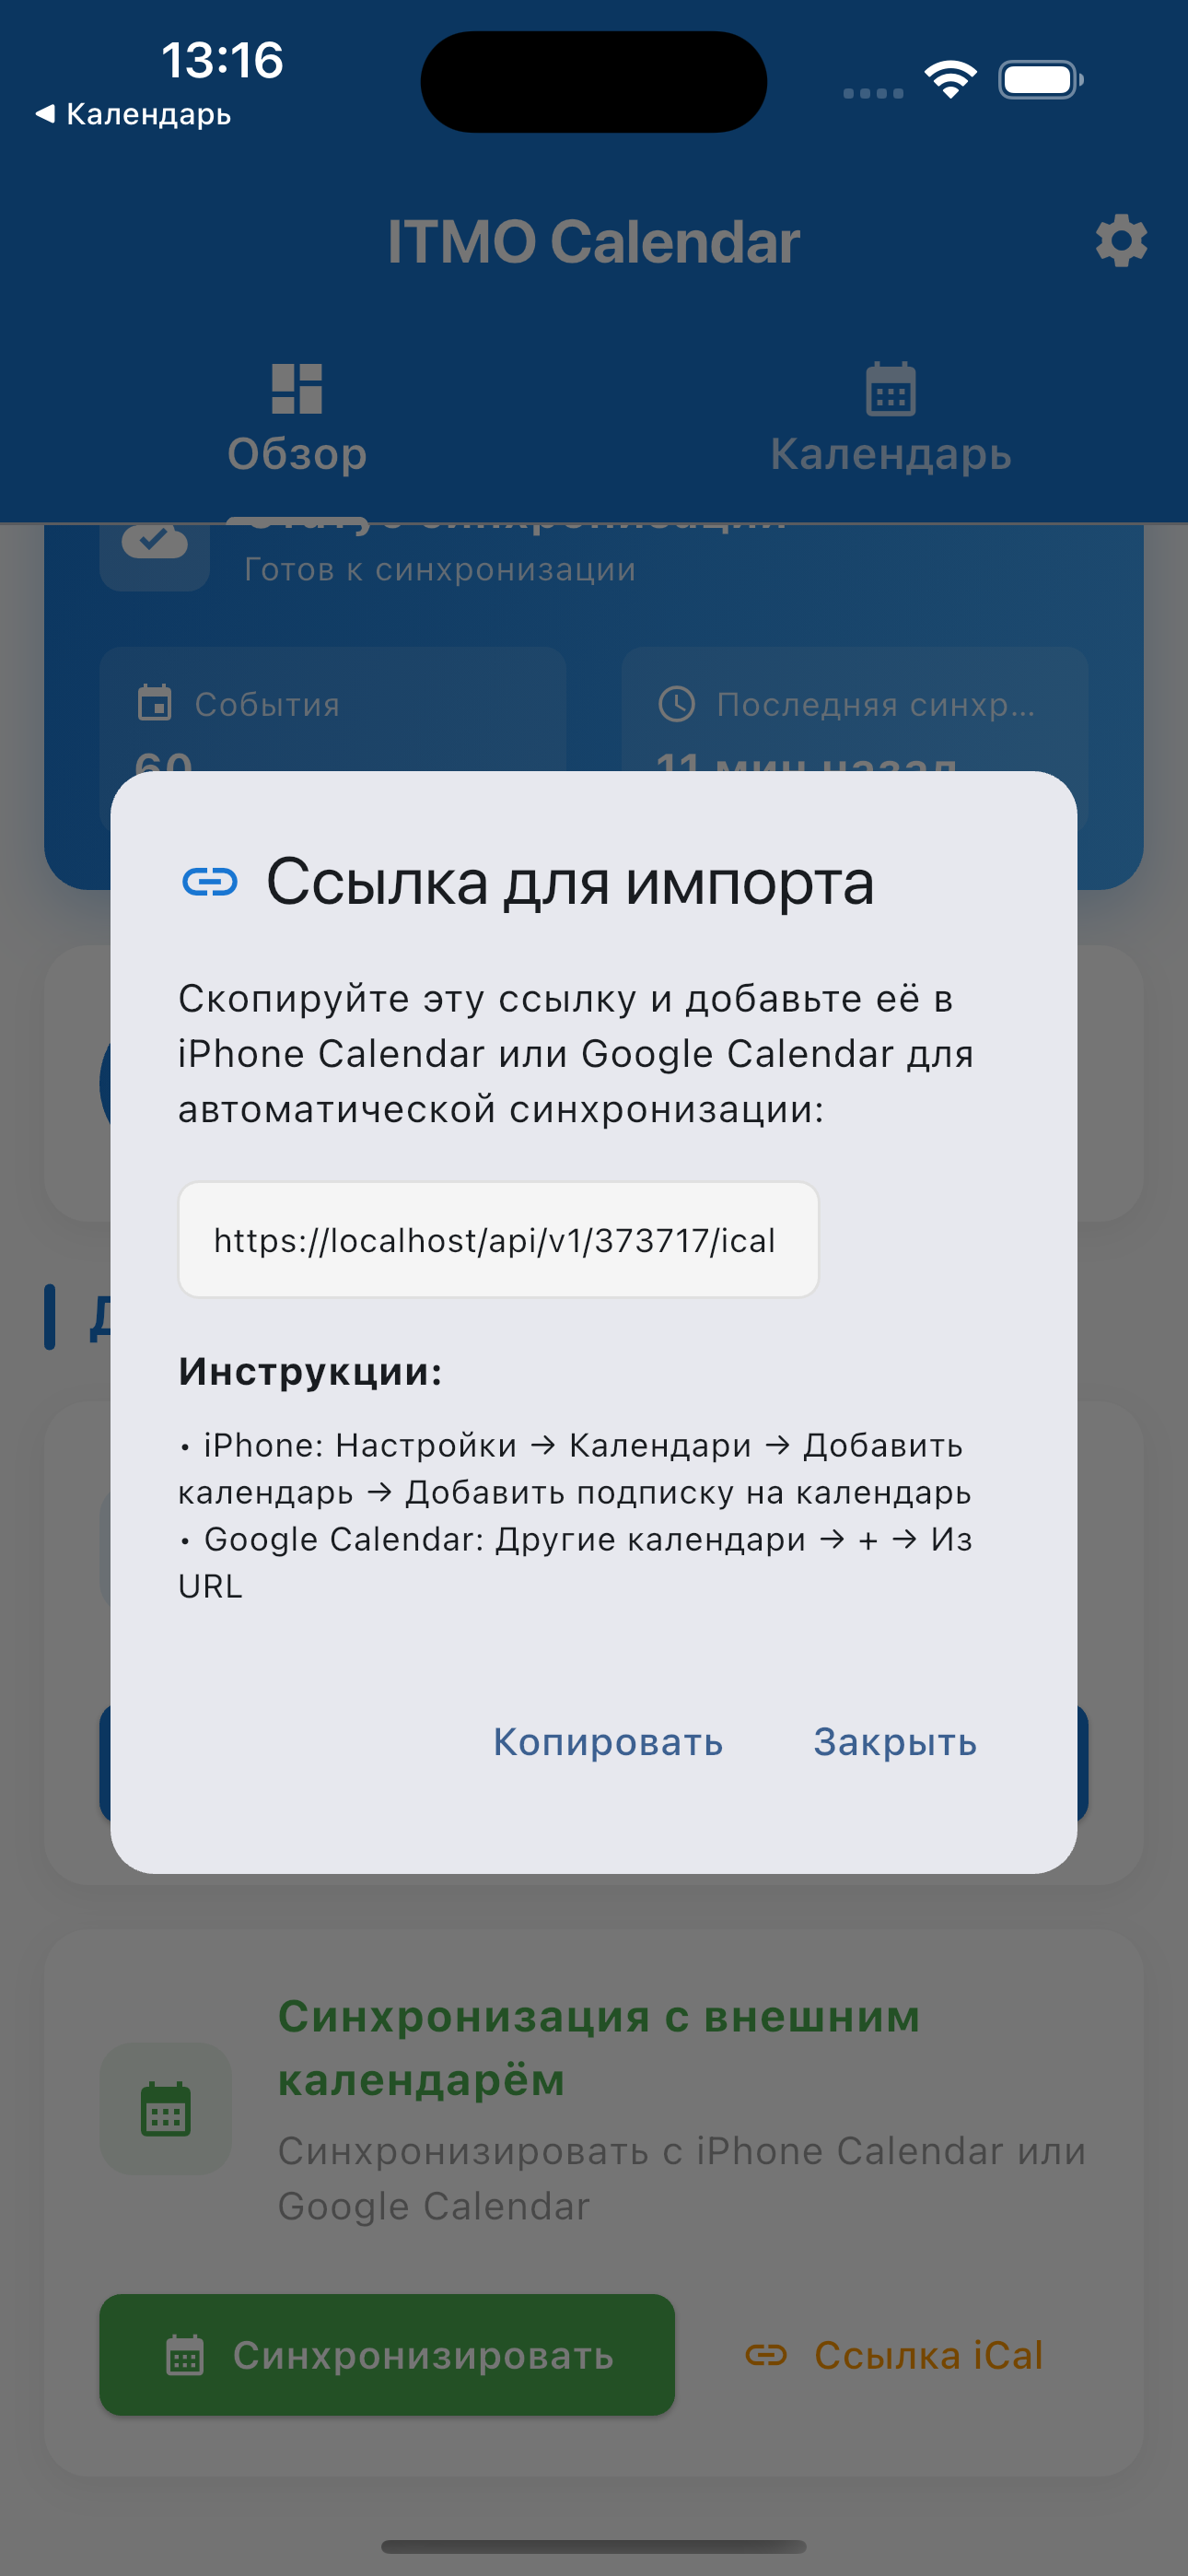
\includegraphics[width=0.6\textwidth]{images/link-for-import-with-instruction.png}
    \caption{Инструкция по импорту календаря}
    \label{fig:import-link}
\end{figure}

\begin{figure}[h!]
    \centering
    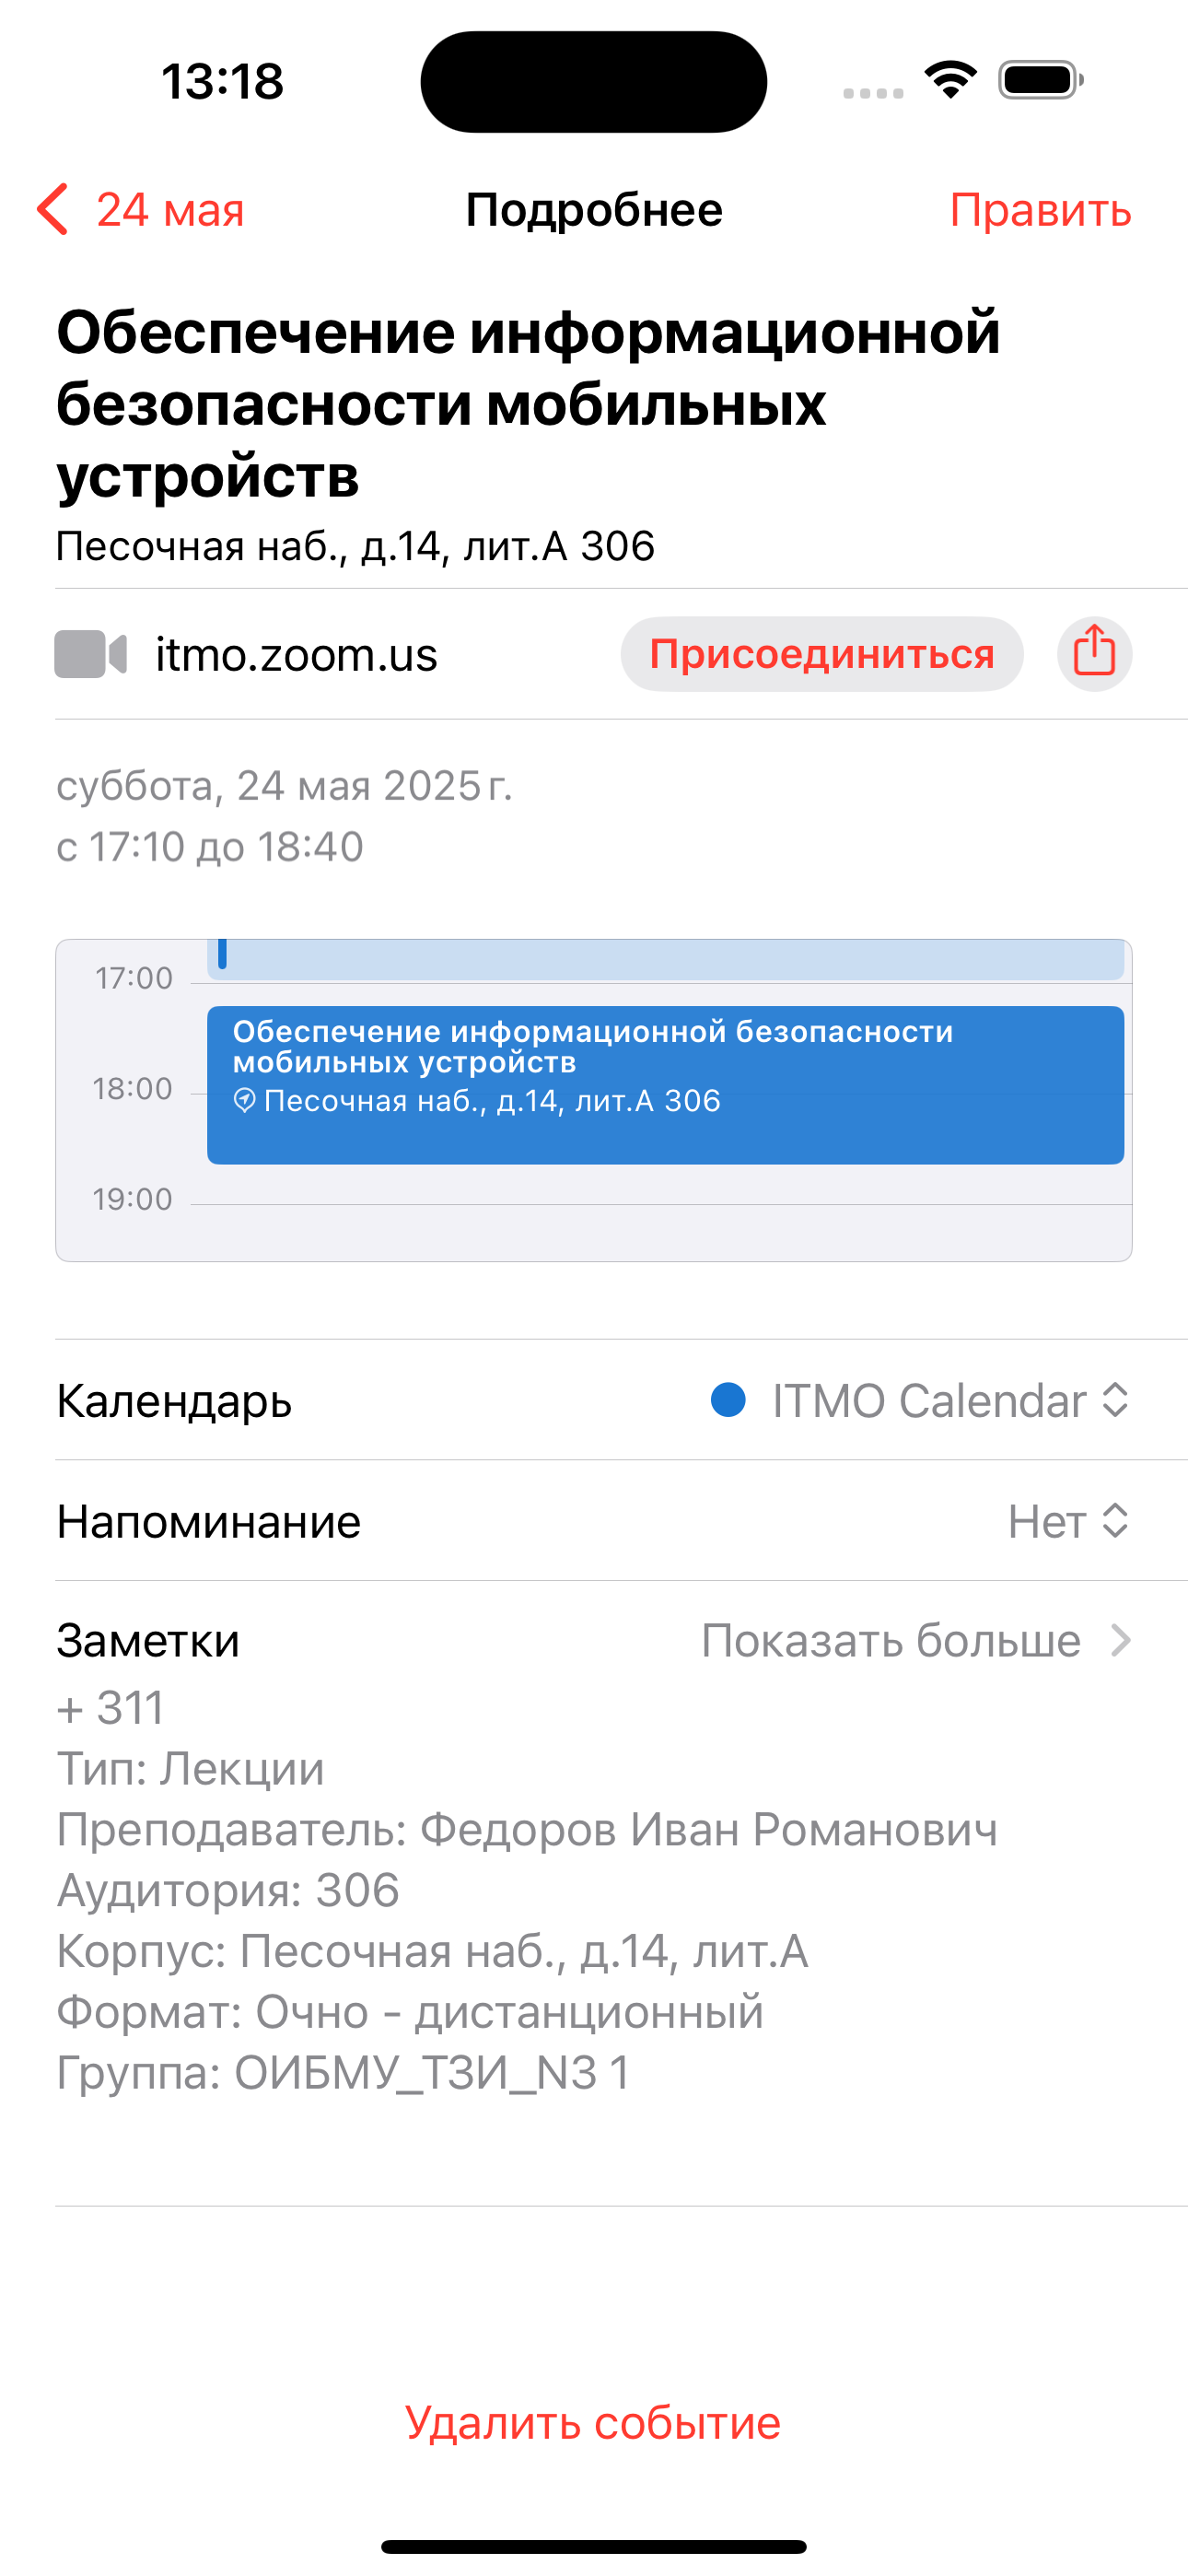
\includegraphics[width=0.6\textwidth]{images/apple-calendar-synced.png}
    \caption{Пример синхронизации с Apple Calendar}
    \label{fig:apple-calendar}
\end{figure}

\chapter*{Заключение}
\addcontentsline{toc}{chapter}{Заключение}

В ходе выполнения данной лабораторной работы была успешно разработана и проанализирована система синхронизации календаря для студентов ИТМО, состоящая из backend-сервиса на языке Go и мобильного приложения на Flutter.

\textbf{Основные результаты работы:}

\begin{enumerate}
    \item \textbf{Backend-сервис itmo-calendar} --- разработан полнофункциональный REST API сервис с использованием современной use-case driven архитектуры. Сервис обеспечивает получение расписания студентов, генерацию iCalendar файлов и подписку пользователей. Реализованы механизмы аутентификации через JWT и поддержка HTTPS для безопасной передачи данных.
    
    \item \textbf{Flutter-приложение calendar-sync} --- создано кроссплатформенное мобильное приложение с современным пользовательским интерфейсом. Приложение использует архитектуру с разделением ответственности, включающую сервисы для работы с API и календарем, провайдеры для управления состоянием и модульную структуру виджетов.
    
    \item \textbf{Механизмы безопасности} --- успешно реализована защита от создания скриншотов с использованием пакета \texttt{screen\_protector}, что предотвращает несанкционированное сохранение содержимого экрана приложения.
    
    \item \textbf{Сетевое взаимодействие} --- обеспечено корректное взаимодействие мобильного приложения с backend API, включая обработку самоподписанных SSL-сертификатов для разработки и настройку HTTP-клиента с таймаутами.
    
    \item \textbf{Анализ безопасности} --- проведен комплексный анализ безопасности разработанного приложения, включающий:
    \begin{itemize}
        \item Сборку APK-файлов с различными настройками обфускации
        \item Декомпиляцию и сравнительный анализ полученных файлов
        \item Сканирование утилитой \texttt{apkleaks} для поиска потенциальных утечек данных
        \item Проверку через сервис VirusTotal на наличие вредоносного кода
    \end{itemize}
    
    \item \textbf{Функциональность приложения} --- реализованы все основные функции календарного приложения: отображение расписания в различных форматах (месяц, неделя, список), настройки синхронизации, генерация ссылок для импорта календаря в сторонние приложения.
\end{enumerate}

\textbf{Выводы по анализу безопасности:}

Проведенный анализ показал, что разработанное приложение соответствует базовым требованиям безопасности. Обфускация кода эффективно усложняет процесс реверс-инжиниринга, а защита от скриншотов предотвращает несанкционированное сохранение конфиденциальной информации. Сканирование специализированными инструментами не выявило критических уязвимостей.


\end{document}
